\documentclass[1p]{elsarticle_modified}
%\bibliographystyle{elsarticle-num}

%\usepackage[colorlinks]{hyperref}
%\usepackage{abbrmath_seonhwa} %\Abb, \Ascr, \Acal ,\Abf, \Afrak
\usepackage{amsfonts}
\usepackage{amssymb}
\usepackage{amsmath}
\usepackage{amsthm}
\usepackage{scalefnt}
\usepackage{amsbsy}
\usepackage{kotex}
\usepackage{caption}
\usepackage{subfig}
\usepackage{color}
\usepackage{graphicx}
\usepackage{xcolor} %% white, black, red, green, blue, cyan, magenta, yellow
\usepackage{float}
\usepackage{setspace}
\usepackage{hyperref}

\usepackage{tikz}
\usetikzlibrary{arrows}

\usepackage{multirow}
\usepackage{array} % fixed length table
\usepackage{hhline}

%%%%%%%%%%%%%%%%%%%%%
\makeatletter
\renewcommand*\env@matrix[1][\arraystretch]{%
	\edef\arraystretch{#1}%
	\hskip -\arraycolsep
	\let\@ifnextchar\new@ifnextchar
	\array{*\c@MaxMatrixCols c}}
\makeatother %https://tex.stackexchange.com/questions/14071/how-can-i-increase-the-line-spacing-in-a-matrix
%%%%%%%%%%%%%%%

\usepackage[normalem]{ulem}

\newcommand{\msout}[1]{\ifmmode\text{\sout{\ensuremath{#1}}}\else\sout{#1}\fi}
%SOURCE: \msout is \stkout macro in https://tex.stackexchange.com/questions/20609/strikeout-in-math-mode

\newcommand{\cancel}[1]{
	\ifmmode
	{\color{red}\msout{#1}}
	\else
	{\color{red}\sout{#1}}
	\fi
}

\newcommand{\add}[1]{
	{\color{blue}\uwave{#1}}
}

\newcommand{\replace}[2]{
	\ifmmode
	{\color{red}\msout{#1}}{\color{blue}\uwave{#2}}
	\else
	{\color{red}\sout{#1}}{\color{blue}\uwave{#2}}
	\fi
}

\newcommand{\Sol}{\mathcal{S}} %segment
\newcommand{\D}{D} %diagram
\newcommand{\A}{\mathcal{A}} %arc


%%%%%%%%%%%%%%%%%%%%%%%%%%%%%5 test

\def\sl{\operatorname{\textup{SL}}(2,\Cbb)}
\def\psl{\operatorname{\textup{PSL}}(2,\Cbb)}
\def\quan{\mkern 1mu \triangleright \mkern 1mu}

\theoremstyle{definition}
\newtheorem{thm}{Theorem}[section]
\newtheorem{prop}[thm]{Proposition}
\newtheorem{lem}[thm]{Lemma}
\newtheorem{ques}[thm]{Question}
\newtheorem{cor}[thm]{Corollary}
\newtheorem{defn}[thm]{Definition}
\newtheorem{exam}[thm]{Example}
\newtheorem{rmk}[thm]{Remark}
\newtheorem{alg}[thm]{Algorithm}

\newcommand{\I}{\sqrt{-1}}
\begin{document}

%\begin{frontmatter}
%
%\title{Boundary parabolic representations of knots up to 8 crossings}
%
%%% Group authors per affiliation:
%\author{Yunhi Cho} 
%\address{Department of Mathematics, University of Seoul, Seoul, Korea}
%\ead{yhcho@uos.ac.kr}
%
%
%\author{Seonhwa Kim} %\fnref{s_kim}}
%\address{Center for Geometry and Physics, Institute for Basic Science, Pohang, 37673, Korea}
%\ead{ryeona17@ibs.re.kr}
%
%\author{Hyuk Kim}
%\address{Department of Mathematical Sciences, Seoul National University, Seoul 08826, Korea}
%\ead{hyukkim@snu.ac.kr}
%
%\author{Seokbeom Yoon}
%\address{Department of Mathematical Sciences, Seoul National University, Seoul, 08826,  Korea}
%\ead{sbyoon15@snu.ac.kr}
%
%\begin{abstract}
%We find all boundary parabolic representation of knots up to 8 crossings.
%
%\end{abstract}
%\begin{keyword}
%    \MSC[2010] 57M25 
%\end{keyword}
%
%\end{frontmatter}

%\linenumbers
%\tableofcontents
%
\newcommand\colored[1]{\textcolor{white}{\rule[-0.35ex]{0.8em}{1.4ex}}\kern-0.8em\color{red} #1}%
%\newcommand\colored[1]{\textcolor{white}{ #1}\kern-2.17ex	\textcolor{white}{ #1}\kern-1.81ex	\textcolor{white}{ #1}\kern-2.15ex\color{red}#1	}

{\Large $\underline{12a_{0700}~(K12a_{0700})}$}

\setlength{\tabcolsep}{10pt}
\renewcommand{\arraystretch}{1.6}
\vspace{1cm}\begin{tabular}{m{100pt}>{\centering\arraybackslash}m{274pt}}
\multirow{5}{120pt}{
	\centering
	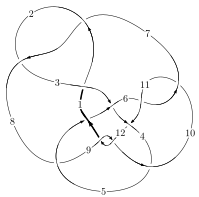
\includegraphics[width=112pt]{../../../GIT/diagram.site/Diagrams/png/1501_12a_0700.png}\\
\ \ \ A knot diagram\footnotemark}&
\allowdisplaybreaks
\textbf{Linearized knot diagam} \\
\cline{2-2}
 &
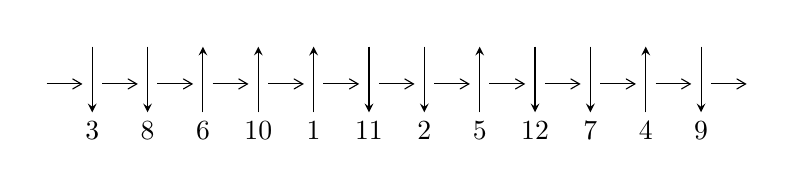
\begin{tikzpicture}[x=20pt, y=17pt]
	% nodes
	\node (C0) at (0, 0) {};
	\node (C1) at (1, 0) {};
	\node (C1U) at (1, +1) {};
	\node (C1D) at (1, -1) {3};

	\node (C2) at (2, 0) {};
	\node (C2U) at (2, +1) {};
	\node (C2D) at (2, -1) {8};

	\node (C3) at (3, 0) {};
	\node (C3U) at (3, +1) {};
	\node (C3D) at (3, -1) {6};

	\node (C4) at (4, 0) {};
	\node (C4U) at (4, +1) {};
	\node (C4D) at (4, -1) {10};

	\node (C5) at (5, 0) {};
	\node (C5U) at (5, +1) {};
	\node (C5D) at (5, -1) {1};

	\node (C6) at (6, 0) {};
	\node (C6U) at (6, +1) {};
	\node (C6D) at (6, -1) {11};

	\node (C7) at (7, 0) {};
	\node (C7U) at (7, +1) {};
	\node (C7D) at (7, -1) {2};

	\node (C8) at (8, 0) {};
	\node (C8U) at (8, +1) {};
	\node (C8D) at (8, -1) {5};

	\node (C9) at (9, 0) {};
	\node (C9U) at (9, +1) {};
	\node (C9D) at (9, -1) {12};

	\node (C10) at (10, 0) {};
	\node (C10U) at (10, +1) {};
	\node (C10D) at (10, -1) {7};

	\node (C11) at (11, 0) {};
	\node (C11U) at (11, +1) {};
	\node (C11D) at (11, -1) {4};

	\node (C12) at (12, 0) {};
	\node (C12U) at (12, +1) {};
	\node (C12D) at (12, -1) {9};
	\node (C13) at (13, 0) {};

	% arrows
	\draw[->,>={angle 60}]
	(C0) edge (C1) (C1) edge (C2) (C2) edge (C3) (C3) edge (C4) (C4) edge (C5) (C5) edge (C6) (C6) edge (C7) (C7) edge (C8) (C8) edge (C9) (C9) edge (C10) (C10) edge (C11) (C11) edge (C12) (C12) edge (C13) ;	\draw[->,>=stealth]
	(C1U) edge (C1D) (C2U) edge (C2D) (C3D) edge (C3U) (C4D) edge (C4U) (C5D) edge (C5U) (C6U) edge (C6D) (C7U) edge (C7D) (C8D) edge (C8U) (C9U) edge (C9D) (C10U) edge (C10D) (C11D) edge (C11U) (C12U) edge (C12D) ;
	\end{tikzpicture} \\
\hhline{~~} \\& 
\textbf{Solving Sequence} \\ \cline{2-2} 
 &
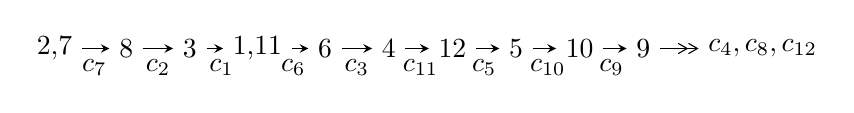
\begin{tikzpicture}[x=23pt, y=7pt]
	% node
	\node (A0) at (-1/8, 0) {2,7};
	\node (A1) at (1, 0) {8};
	\node (A2) at (2, 0) {3};
	\node (A3) at (49/16, 0) {1,11};
	\node (A4) at (33/8, 0) {6};
	\node (A5) at (41/8, 0) {4};
	\node (A6) at (49/8, 0) {12};
	\node (A7) at (57/8, 0) {5};
	\node (A8) at (65/8, 0) {10};
	\node (A9) at (73/8, 0) {9};
	\node (C1) at (1/2, -1) {$c_{7}$};
	\node (C2) at (3/2, -1) {$c_{2}$};
	\node (C3) at (5/2, -1) {$c_{1}$};
	\node (C4) at (29/8, -1) {$c_{6}$};
	\node (C5) at (37/8, -1) {$c_{3}$};
	\node (C6) at (45/8, -1) {$c_{11}$};
	\node (C7) at (53/8, -1) {$c_{5}$};
	\node (C8) at (61/8, -1) {$c_{10}$};
	\node (C9) at (69/8, -1) {$c_{9}$};
	\node (A10) at (11, 0) {$c_{4},c_{8},c_{12}$};

	% edge
	\draw[->,>=stealth]	
	(A0) edge (A1) (A1) edge (A2) (A2) edge (A3) (A3) edge (A4) (A4) edge (A5) (A5) edge (A6) (A6) edge (A7) (A7) edge (A8) (A8) edge (A9) ;
	\draw[->>,>={angle 60}]	
	(A9) edge (A10);
\end{tikzpicture} \\ 

\end{tabular} \\

\footnotetext{
The image of knot diagram is generated by the software ``\textbf{Draw programme}" developed by Andrew Bartholomew(\url{http://www.layer8.co.uk/maths/draw/index.htm\#Running-draw}), where we modified some parts for our purpose(\url{https://github.com/CATsTAILs/LinksPainter}).
}\phantom \\ \newline 
\centering \textbf{Ideals for irreducible components\footnotemark of $X_{\text{par}}$} 
 
\begin{align*}
I^u_{1}&=\langle 
1.67707\times10^{517} u^{170}+2.41772\times10^{516} u^{169}+\cdots+4.22459\times10^{515} b+4.07568\times10^{519},\\
\phantom{I^u_{1}}&\phantom{= \langle  }-1.58770\times10^{520} u^{170}+3.63892\times10^{519} u^{169}+\cdots+1.67716\times10^{518} a-6.29761\times10^{522},\\
\phantom{I^u_{1}}&\phantom{= \langle  }u^{171}- u^{170}+\cdots+586 u-397\rangle \\
I^u_{2}&=\langle 
-205536567 u^{44}+2638046874 u^{43}+\cdots+279594103 b-13616934025,\\
\phantom{I^u_{2}}&\phantom{= \langle  }-12067050844 u^{44}-2918818158 u^{43}+\cdots+838782309 a-5408626830,\\
\phantom{I^u_{2}}&\phantom{= \langle  }u^{45}-14 u^{43}+\cdots-9 u+3\rangle \\
\\
\end{align*}
\raggedright * 2 irreducible components of $\dim_{\mathbb{C}}=0$, with total 216 representations.\\
\footnotetext{All coefficients of polynomials are rational numbers. But the coefficients are sometimes approximated in decimal forms when there is not enough margin.}
\newpage
\renewcommand{\arraystretch}{1}
\centering \section*{I. $I^u_{1}= \langle 1.68\times10^{517} u^{170}+2.42\times10^{516} u^{169}+\cdots+4.22\times10^{515} b+4.08\times10^{519},\;-1.59\times10^{520} u^{170}+3.64\times10^{519} u^{169}+\cdots+1.68\times10^{518} a-6.30\times10^{522},\;u^{171}- u^{170}+\cdots+586 u-397 \rangle$}
\flushleft \textbf{(i) Arc colorings}\\
\begin{tabular}{m{7pt} m{180pt} m{7pt} m{180pt} }
\flushright $a_{2}=$&$\begin{pmatrix}0\\u\end{pmatrix}$ \\
\flushright $a_{7}=$&$\begin{pmatrix}1\\0\end{pmatrix}$ \\
\flushright $a_{8}=$&$\begin{pmatrix}1\\u^2\end{pmatrix}$ \\
\flushright $a_{3}=$&$\begin{pmatrix}- u\\- u^3+u\end{pmatrix}$ \\
\flushright $a_{1}=$&$\begin{pmatrix}u^3\\u^5- u^3+u\end{pmatrix}$ \\
\flushright $a_{11}=$&$\begin{pmatrix}94.6662 u^{170}-21.6969 u^{169}+\cdots-26585.7 u+37549.3\\-39.6979 u^{170}-5.72299 u^{169}+\cdots+13115.3 u-9647.53\end{pmatrix}$ \\
\flushright $a_{6}=$&$\begin{pmatrix}45.9599 u^{170}-17.2381 u^{169}+\cdots-12547.3 u+20732.1\\-24.4709 u^{170}-5.37117 u^{169}+\cdots+8344.75 u-4907.67\end{pmatrix}$ \\
\flushright $a_{4}=$&$\begin{pmatrix}11.3771 u^{170}-0.208651 u^{169}+\cdots-3186.44 u+3718.02\\-3.07513 u^{170}-1.79771 u^{169}+\cdots+1127.40 u-259.968\end{pmatrix}$ \\
\flushright $a_{12}=$&$\begin{pmatrix}29.4345 u^{170}-32.1297 u^{169}+\cdots-4225.62 u+22195.0\\-32.0724 u^{170}-1.34218 u^{169}+\cdots+10101.1 u-9251.27\end{pmatrix}$ \\
\flushright $a_{5}=$&$\begin{pmatrix}24.1839 u^{170}-23.7891 u^{169}+\cdots-4829.20 u+17221.1\\-24.8459 u^{170}-7.07327 u^{169}+\cdots+8647.31 u-4301.28\end{pmatrix}$ \\
\flushright $a_{10}=$&$\begin{pmatrix}54.9682 u^{170}-27.4199 u^{169}+\cdots-13470.4 u+27901.7\\-39.6979 u^{170}-5.72299 u^{169}+\cdots+13115.3 u-9647.53\end{pmatrix}$ \\
\flushright $a_{9}=$&$\begin{pmatrix}-10.9228 u^{170}-8.36188 u^{169}+\cdots+4785.16 u-94.6923\\-19.2601 u^{170}+3.11046 u^{169}+\cdots+5477.55 u-7237.79\end{pmatrix}$\\&\end{tabular}
\flushleft \textbf{(ii) Obstruction class $= -1$}\\~\\
\flushleft \textbf{(iii) Cusp Shapes $= 61.8148 u^{170}+26.9336 u^{169}+\cdots-21906.6 u+8391.20$}\\~\\
\newpage\renewcommand{\arraystretch}{1}
\flushleft \textbf{(iv) u-Polynomials at the component}\newline \\
\begin{tabular}{m{50pt}|m{274pt}}
Crossings & \hspace{64pt}u-Polynomials at each crossing \\
\hline $$\begin{aligned}c_{1}\end{aligned}$$&$\begin{aligned}
&u^{171}+79 u^{170}+\cdots+1899636 u+157609
\end{aligned}$\\
\hline $$\begin{aligned}c_{2},c_{7}\end{aligned}$$&$\begin{aligned}
&u^{171}- u^{170}+\cdots+586 u-397
\end{aligned}$\\
\hline $$\begin{aligned}c_{3}\end{aligned}$$&$\begin{aligned}
&u^{171}-16 u^{170}+\cdots-105850260074 u+6222620143
\end{aligned}$\\
\hline $$\begin{aligned}c_{4}\end{aligned}$$&$\begin{aligned}
&u^{171}+u^{170}+\cdots+6244268 u+1871863
\end{aligned}$\\
\hline $$\begin{aligned}c_{5}\end{aligned}$$&$\begin{aligned}
&u^{171}-24 u^{169}+\cdots-319818841 u-22221569
\end{aligned}$\\
\hline $$\begin{aligned}c_{6},c_{10}\end{aligned}$$&$\begin{aligned}
&u^{171}+2 u^{170}+\cdots-92496 u-62927
\end{aligned}$\\
\hline $$\begin{aligned}c_{8}\end{aligned}$$&$\begin{aligned}
&u^{171}-5 u^{170}+\cdots+7769088 u+837632
\end{aligned}$\\
\hline $$\begin{aligned}c_{9},c_{12}\end{aligned}$$&$\begin{aligned}
&u^{171}-6 u^{170}+\cdots-48 u+1
\end{aligned}$\\
\hline $$\begin{aligned}c_{11}\end{aligned}$$&$\begin{aligned}
&u^{171}-3 u^{170}+\cdots-5954691744 u+869790560
\end{aligned}$\\
\hline
\end{tabular}\\~\\
\newpage\renewcommand{\arraystretch}{1}
\flushleft \textbf{(v) Riley Polynomials at the component}\newline \\
\begin{tabular}{m{50pt}|m{274pt}}
Crossings & \hspace{64pt}Riley Polynomials at each crossing \\
\hline $$\begin{aligned}c_{1}\end{aligned}$$&$\begin{aligned}
&y^{171}+41 y^{170}+\cdots+2670305620588 y-24840596881
\end{aligned}$\\
\hline $$\begin{aligned}c_{2},c_{7}\end{aligned}$$&$\begin{aligned}
&y^{171}-79 y^{170}+\cdots+1899636 y-157609
\end{aligned}$\\
\hline $$\begin{aligned}c_{3}\end{aligned}$$&$\begin{aligned}
&y^{171}-60 y^{170}+\cdots+3.41\times10^{21} y-3.87\times10^{19}
\end{aligned}$\\
\hline $$\begin{aligned}c_{4}\end{aligned}$$&$\begin{aligned}
&y^{171}-39 y^{170}+\cdots+212094663334992 y-3503871090769
\end{aligned}$\\
\hline $$\begin{aligned}c_{5}\end{aligned}$$&$\begin{aligned}
&y^{171}-48 y^{170}+\cdots+23054962778381399 y-493798128821761
\end{aligned}$\\
\hline $$\begin{aligned}c_{6},c_{10}\end{aligned}$$&$\begin{aligned}
&y^{171}+100 y^{170}+\cdots-122657730866 y-3959807329
\end{aligned}$\\
\hline $$\begin{aligned}c_{8}\end{aligned}$$&$\begin{aligned}
&y^{171}-29 y^{170}+\cdots+26226872811520 y-701627367424
\end{aligned}$\\
\hline $$\begin{aligned}c_{9},c_{12}\end{aligned}$$&$\begin{aligned}
&y^{171}+124 y^{170}+\cdots+6 y-1
\end{aligned}$\\
\hline $$\begin{aligned}c_{11}\end{aligned}$$&$\begin{aligned}
&y^{171}-61 y^{170}+\cdots+5.18\times10^{19} y-7.57\times10^{17}
\end{aligned}$\\
\hline
\end{tabular}\\~\\
\newpage\flushleft \textbf{(vi) Complex Volumes and Cusp Shapes}
$$\begin{array}{c|c|c}  
\text{Solutions to }I^u_{1}& \I (\text{vol} + \sqrt{-1}CS) & \text{Cusp shape}\\
 \hline 
\begin{aligned}
u &= \phantom{-}0.956826 + 0.287603 I \\
a &= -0.214990 + 0.039118 I \\
b &= \phantom{-}0.617261 - 1.256480 I\end{aligned}
 & \phantom{-}2.51554 + 4.66422 I & \phantom{-0.000000 } 0 \\ \hline\begin{aligned}
u &= \phantom{-}0.956826 - 0.287603 I \\
a &= -0.214990 - 0.039118 I \\
b &= \phantom{-}0.617261 + 1.256480 I\end{aligned}
 & \phantom{-}2.51554 - 4.66422 I & \phantom{-0.000000 } 0 \\ \hline\begin{aligned}
u &= \phantom{-}0.878636 + 0.466670 I \\
a &= -1.81779 + 3.02433 I \\
b &= -0.127767 - 0.933514 I\end{aligned}
 & -2.23105 - 1.90040 I & \phantom{-0.000000 } 0 \\ \hline\begin{aligned}
u &= \phantom{-}0.878636 - 0.466670 I \\
a &= -1.81779 - 3.02433 I \\
b &= -0.127767 + 0.933514 I\end{aligned}
 & -2.23105 + 1.90040 I & \phantom{-0.000000 } 0 \\ \hline\begin{aligned}
u &= -0.797590 + 0.613927 I \\
a &= \phantom{-}0.36054 + 1.81675 I \\
b &= -0.495385 - 1.175970 I\end{aligned}
 & \phantom{-}7.74690 + 0.58892 I & \phantom{-0.000000 } 0 \\ \hline\begin{aligned}
u &= -0.797590 - 0.613927 I \\
a &= \phantom{-}0.36054 - 1.81675 I \\
b &= -0.495385 + 1.175970 I\end{aligned}
 & \phantom{-}7.74690 - 0.58892 I & \phantom{-0.000000 } 0 \\ \hline\begin{aligned}
u &= \phantom{-}0.897140 + 0.461300 I \\
a &= -0.222009 - 1.350370 I \\
b &= \phantom{-}1.236070 + 0.216738 I\end{aligned}
 & -1.24696 - 4.30194 I & \phantom{-0.000000 } 0 \\ \hline\begin{aligned}
u &= \phantom{-}0.897140 - 0.461300 I \\
a &= -0.222009 + 1.350370 I \\
b &= \phantom{-}1.236070 - 0.216738 I\end{aligned}
 & -1.24696 + 4.30194 I & \phantom{-0.000000 } 0 \\ \hline\begin{aligned}
u &= \phantom{-}0.868052 + 0.461448 I \\
a &= \phantom{-}0.76462 + 1.23283 I \\
b &= -1.314450 + 0.413646 I\end{aligned}
 & -1.156070 + 0.546217 I & \phantom{-0.000000 } 0 \\ \hline\begin{aligned}
u &= \phantom{-}0.868052 - 0.461448 I \\
a &= \phantom{-}0.76462 - 1.23283 I \\
b &= -1.314450 - 0.413646 I\end{aligned}
 & -1.156070 - 0.546217 I & \phantom{-0.000000 } 0\\
 \hline 
 \end{array}$$\newpage$$\begin{array}{c|c|c}  
\text{Solutions to }I^u_{1}& \I (\text{vol} + \sqrt{-1}CS) & \text{Cusp shape}\\
 \hline 
\begin{aligned}
u &= \phantom{-}0.975014 + 0.100724 I \\
a &= -0.197692 - 0.624980 I \\
b &= -0.324228 + 1.176300 I\end{aligned}
 & \phantom{-}4.48921 + 2.47656 I & \phantom{-0.000000 } 0 \\ \hline\begin{aligned}
u &= \phantom{-}0.975014 - 0.100724 I \\
a &= -0.197692 + 0.624980 I \\
b &= -0.324228 - 1.176300 I\end{aligned}
 & \phantom{-}4.48921 - 2.47656 I & \phantom{-0.000000 } 0 \\ \hline\begin{aligned}
u &= -0.546543 + 0.862927 I \\
a &= -0.257752 + 0.432459 I \\
b &= \phantom{-}1.257840 - 0.106489 I\end{aligned}
 & \phantom{-}0.67913 - 2.32400 I & \phantom{-0.000000 } 0 \\ \hline\begin{aligned}
u &= -0.546543 - 0.862927 I \\
a &= -0.257752 - 0.432459 I \\
b &= \phantom{-}1.257840 + 0.106489 I\end{aligned}
 & \phantom{-}0.67913 + 2.32400 I & \phantom{-0.000000 } 0 \\ \hline\begin{aligned}
u &= -0.491789 + 0.845790 I \\
a &= \phantom{-}0.401471 - 0.341501 I \\
b &= -1.148200 + 0.080607 I\end{aligned}
 & \phantom{-}5.73401 - 8.33723 I & \phantom{-0.000000 } 0 \\ \hline\begin{aligned}
u &= -0.491789 - 0.845790 I \\
a &= \phantom{-}0.401471 + 0.341501 I \\
b &= -1.148200 - 0.080607 I\end{aligned}
 & \phantom{-}5.73401 + 8.33723 I & \phantom{-0.000000 } 0 \\ \hline\begin{aligned}
u &= -0.608462 + 0.761738 I \\
a &= \phantom{-}0.47379 + 2.13450 I \\
b &= -0.297301 - 1.222780 I\end{aligned}
 & \phantom{-}5.48470 - 3.12328 I & \phantom{-0.000000 } 0 \\ \hline\begin{aligned}
u &= -0.608462 - 0.761738 I \\
a &= \phantom{-}0.47379 - 2.13450 I \\
b &= -0.297301 + 1.222780 I\end{aligned}
 & \phantom{-}5.48470 + 3.12328 I & \phantom{-0.000000 } 0 \\ \hline\begin{aligned}
u &= \phantom{-}0.934716 + 0.439830 I \\
a &= \phantom{-}2.64369 - 1.69700 I \\
b &= \phantom{-}0.224833 + 0.839728 I\end{aligned}
 & \phantom{-}1.55184 - 5.66028 I & \phantom{-0.000000 } 0 \\ \hline\begin{aligned}
u &= \phantom{-}0.934716 - 0.439830 I \\
a &= \phantom{-}2.64369 + 1.69700 I \\
b &= \phantom{-}0.224833 - 0.839728 I\end{aligned}
 & \phantom{-}1.55184 + 5.66028 I & \phantom{-0.000000 } 0\\
 \hline 
 \end{array}$$\newpage$$\begin{array}{c|c|c}  
\text{Solutions to }I^u_{1}& \I (\text{vol} + \sqrt{-1}CS) & \text{Cusp shape}\\
 \hline 
\begin{aligned}
u &= \phantom{-}1.026210 + 0.132140 I \\
a &= \phantom{-}0.94526 - 1.12379 I \\
b &= \phantom{-}0.682948 + 0.550960 I\end{aligned}
 & -2.33748 - 4.36060 I & \phantom{-0.000000 } 0 \\ \hline\begin{aligned}
u &= \phantom{-}1.026210 - 0.132140 I \\
a &= \phantom{-}0.94526 + 1.12379 I \\
b &= \phantom{-}0.682948 - 0.550960 I\end{aligned}
 & -2.33748 + 4.36060 I & \phantom{-0.000000 } 0 \\ \hline\begin{aligned}
u &= \phantom{-}0.853301 + 0.448186 I \\
a &= \phantom{-}0.83149 - 3.63508 I \\
b &= \phantom{-}0.078705 + 0.937908 I\end{aligned}
 & \phantom{-}1.80141 + 2.02979 I & \phantom{-0.000000 } 0 \\ \hline\begin{aligned}
u &= \phantom{-}0.853301 - 0.448186 I \\
a &= \phantom{-}0.83149 + 3.63508 I \\
b &= \phantom{-}0.078705 - 0.937908 I\end{aligned}
 & \phantom{-}1.80141 - 2.02979 I & \phantom{-0.000000 } 0 \\ \hline\begin{aligned}
u &= -0.459919 + 0.838834 I \\
a &= \phantom{-}0.003273 - 0.141996 I \\
b &= -1.007690 + 0.303161 I\end{aligned}
 & \phantom{-}5.64380 + 4.62745 I & \phantom{-0.000000 } 0 \\ \hline\begin{aligned}
u &= -0.459919 - 0.838834 I \\
a &= \phantom{-}0.003273 + 0.141996 I \\
b &= -1.007690 - 0.303161 I\end{aligned}
 & \phantom{-}5.64380 - 4.62745 I & \phantom{-0.000000 } 0 \\ \hline\begin{aligned}
u &= -0.921616 + 0.490534 I \\
a &= -0.735283 - 0.208805 I \\
b &= -0.550307 - 0.688727 I\end{aligned}
 & -1.89895 + 2.67491 I & \phantom{-0.000000 } 0 \\ \hline\begin{aligned}
u &= -0.921616 - 0.490534 I \\
a &= -0.735283 + 0.208805 I \\
b &= -0.550307 + 0.688727 I\end{aligned}
 & -1.89895 - 2.67491 I & \phantom{-0.000000 } 0 \\ \hline\begin{aligned}
u &= -0.907689 + 0.517824 I \\
a &= -0.92556 - 1.31095 I \\
b &= -1.165630 + 0.699508 I\end{aligned}
 & -0.69875 + 4.90531 I & \phantom{-0.000000 } 0 \\ \hline\begin{aligned}
u &= -0.907689 - 0.517824 I \\
a &= -0.92556 + 1.31095 I \\
b &= -1.165630 - 0.699508 I\end{aligned}
 & -0.69875 - 4.90531 I & \phantom{-0.000000 } 0\\
 \hline 
 \end{array}$$\newpage$$\begin{array}{c|c|c}  
\text{Solutions to }I^u_{1}& \I (\text{vol} + \sqrt{-1}CS) & \text{Cusp shape}\\
 \hline 
\begin{aligned}
u &= -0.877483 + 0.376347 I \\
a &= \phantom{-}0.667543 + 0.222189 I \\
b &= \phantom{-}0.671106 - 0.312724 I\end{aligned}
 & -1.40660 + 0.95422 I & \phantom{-0.000000 } 0 \\ \hline\begin{aligned}
u &= -0.877483 - 0.376347 I \\
a &= \phantom{-}0.667543 - 0.222189 I \\
b &= \phantom{-}0.671106 + 0.312724 I\end{aligned}
 & -1.40660 - 0.95422 I & \phantom{-0.000000 } 0 \\ \hline\begin{aligned}
u &= -0.900009 + 0.536045 I \\
a &= \phantom{-}1.356680 - 0.146144 I \\
b &= \phantom{-}0.456857 + 0.768723 I\end{aligned}
 & \phantom{-}2.43989 + 6.24179 I & \phantom{-0.000000 } 0 \\ \hline\begin{aligned}
u &= -0.900009 - 0.536045 I \\
a &= \phantom{-}1.356680 + 0.146144 I \\
b &= \phantom{-}0.456857 - 0.768723 I\end{aligned}
 & \phantom{-}2.43989 - 6.24179 I & \phantom{-0.000000 } 0 \\ \hline\begin{aligned}
u &= -0.789179 + 0.530446 I \\
a &= -1.53402 + 0.29766 I \\
b &= -0.532062 + 0.537487 I\end{aligned}
 & \phantom{-}2.78965 - 1.92572 I & \phantom{-0.000000 } 0 \\ \hline\begin{aligned}
u &= -0.789179 - 0.530446 I \\
a &= -1.53402 - 0.29766 I \\
b &= -0.532062 - 0.537487 I\end{aligned}
 & \phantom{-}2.78965 + 1.92572 I & \phantom{-0.000000 } 0 \\ \hline\begin{aligned}
u &= \phantom{-}0.448529 + 0.949574 I \\
a &= -0.00572 - 1.62100 I \\
b &= -0.57346 + 1.34895 I\end{aligned}
 & \phantom{-}9.7363 + 14.3889 I & \phantom{-0.000000 } 0 \\ \hline\begin{aligned}
u &= \phantom{-}0.448529 - 0.949574 I \\
a &= -0.00572 + 1.62100 I \\
b &= -0.57346 - 1.34895 I\end{aligned}
 & \phantom{-}9.7363 - 14.3889 I & \phantom{-0.000000 } 0 \\ \hline\begin{aligned}
u &= \phantom{-}0.355744 + 0.993600 I \\
a &= -0.142783 - 1.263270 I \\
b &= -0.66863 + 1.35759 I\end{aligned}
 & \phantom{-}8.71974 + 1.76736 I & \phantom{-0.000000 } 0 \\ \hline\begin{aligned}
u &= \phantom{-}0.355744 - 0.993600 I \\
a &= -0.142783 + 1.263270 I \\
b &= -0.66863 - 1.35759 I\end{aligned}
 & \phantom{-}8.71974 - 1.76736 I & \phantom{-0.000000 } 0\\
 \hline 
 \end{array}$$\newpage$$\begin{array}{c|c|c}  
\text{Solutions to }I^u_{1}& \I (\text{vol} + \sqrt{-1}CS) & \text{Cusp shape}\\
 \hline 
\begin{aligned}
u &= \phantom{-}0.657732 + 0.829253 I \\
a &= -0.62813 + 1.85085 I \\
b &= -0.41368 - 1.49142 I\end{aligned}
 & \phantom{-}10.95280 + 2.50693 I & \phantom{-0.000000 } 0 \\ \hline\begin{aligned}
u &= \phantom{-}0.657732 - 0.829253 I \\
a &= -0.62813 - 1.85085 I \\
b &= -0.41368 + 1.49142 I\end{aligned}
 & \phantom{-}10.95280 - 2.50693 I & \phantom{-0.000000 } 0 \\ \hline\begin{aligned}
u &= -0.423891 + 0.974839 I \\
a &= \phantom{-}0.09072 - 1.71356 I \\
b &= \phantom{-}0.099083 + 1.055390 I\end{aligned}
 & \phantom{-}3.39888 - 0.77235 I & \phantom{-0.000000 } 0 \\ \hline\begin{aligned}
u &= -0.423891 - 0.974839 I \\
a &= \phantom{-}0.09072 + 1.71356 I \\
b &= \phantom{-}0.099083 - 1.055390 I\end{aligned}
 & \phantom{-}3.39888 + 0.77235 I & \phantom{-0.000000 } 0 \\ \hline\begin{aligned}
u &= \phantom{-}0.444365 + 0.969023 I \\
a &= -0.02205 + 1.50059 I \\
b &= \phantom{-}0.57395 - 1.36722 I\end{aligned}
 & \phantom{-}4.81458 + 8.62639 I & \phantom{-0.000000 } 0 \\ \hline\begin{aligned}
u &= \phantom{-}0.444365 - 0.969023 I \\
a &= -0.02205 - 1.50059 I \\
b &= \phantom{-}0.57395 + 1.36722 I\end{aligned}
 & \phantom{-}4.81458 - 8.62639 I & \phantom{-0.000000 } 0 \\ \hline\begin{aligned}
u &= \phantom{-}0.863125 + 0.350401 I \\
a &= \phantom{-}0.238619 + 0.673714 I \\
b &= -0.722226 + 1.021860 I\end{aligned}
 & \phantom{-}0.55593 + 1.81783 I & \phantom{-0.000000 } 0 \\ \hline\begin{aligned}
u &= \phantom{-}0.863125 - 0.350401 I \\
a &= \phantom{-}0.238619 - 0.673714 I \\
b &= -0.722226 - 1.021860 I\end{aligned}
 & \phantom{-}0.55593 - 1.81783 I & \phantom{-0.000000 } 0 \\ \hline\begin{aligned}
u &= \phantom{-}0.419292 + 0.829504 I \\
a &= \phantom{-}0.083582 + 0.849301 I \\
b &= -0.212142 - 0.509063 I\end{aligned}
 & \phantom{-}3.81399 + 2.47640 I & \phantom{-0.000000 } 0 \\ \hline\begin{aligned}
u &= \phantom{-}0.419292 - 0.829504 I \\
a &= \phantom{-}0.083582 - 0.849301 I \\
b &= -0.212142 + 0.509063 I\end{aligned}
 & \phantom{-}3.81399 - 2.47640 I & \phantom{-0.000000 } 0\\
 \hline 
 \end{array}$$\newpage$$\begin{array}{c|c|c}  
\text{Solutions to }I^u_{1}& \I (\text{vol} + \sqrt{-1}CS) & \text{Cusp shape}\\
 \hline 
\begin{aligned}
u &= -0.893807 + 0.590700 I \\
a &= \phantom{-}1.98942 + 2.00045 I \\
b &= \phantom{-}0.599518 - 1.103710 I\end{aligned}
 & \phantom{-}7.44851 + 4.15937 I & \phantom{-0.000000 } 0 \\ \hline\begin{aligned}
u &= -0.893807 - 0.590700 I \\
a &= \phantom{-}1.98942 - 2.00045 I \\
b &= \phantom{-}0.599518 + 1.103710 I\end{aligned}
 & \phantom{-}7.44851 - 4.15937 I & \phantom{-0.000000 } 0 \\ \hline\begin{aligned}
u &= -0.731601 + 0.786359 I \\
a &= -0.60679 - 1.96764 I \\
b &= \phantom{-}0.402401 + 1.167230 I\end{aligned}
 & \phantom{-}8.68265 - 3.67599 I & \phantom{-0.000000 } 0 \\ \hline\begin{aligned}
u &= -0.731601 - 0.786359 I \\
a &= -0.60679 + 1.96764 I \\
b &= \phantom{-}0.402401 - 1.167230 I\end{aligned}
 & \phantom{-}8.68265 + 3.67599 I & \phantom{-0.000000 } 0 \\ \hline\begin{aligned}
u &= -0.997567 + 0.422352 I \\
a &= \phantom{-}0.318505 + 0.536245 I \\
b &= \phantom{-}0.916995 - 0.035295 I\end{aligned}
 & -1.11246 + 1.02477 I & \phantom{-0.000000 } 0 \\ \hline\begin{aligned}
u &= -0.997567 - 0.422352 I \\
a &= \phantom{-}0.318505 - 0.536245 I \\
b &= \phantom{-}0.916995 + 0.035295 I\end{aligned}
 & -1.11246 - 1.02477 I & \phantom{-0.000000 } 0 \\ \hline\begin{aligned}
u &= -0.715901 + 0.558446 I \\
a &= -0.96085 - 1.69301 I \\
b &= \phantom{-}0.53387 + 1.35453 I\end{aligned}
 & \phantom{-}2.74819 - 2.02548 I & \phantom{-0.000000 } 0 \\ \hline\begin{aligned}
u &= -0.715901 - 0.558446 I \\
a &= -0.96085 + 1.69301 I \\
b &= \phantom{-}0.53387 - 1.35453 I\end{aligned}
 & \phantom{-}2.74819 + 2.02548 I & \phantom{-0.000000 } 0 \\ \hline\begin{aligned}
u &= -0.769705 + 0.481037 I \\
a &= -0.205971 + 0.066204 I \\
b &= \phantom{-}0.928769 + 0.717151 I\end{aligned}
 & -0.257115 - 0.769190 I & \phantom{-0.000000 } 0 \\ \hline\begin{aligned}
u &= -0.769705 - 0.481037 I \\
a &= -0.205971 - 0.066204 I \\
b &= \phantom{-}0.928769 - 0.717151 I\end{aligned}
 & -0.257115 + 0.769190 I & \phantom{-0.000000 } 0\\
 \hline 
 \end{array}$$\newpage$$\begin{array}{c|c|c}  
\text{Solutions to }I^u_{1}& \I (\text{vol} + \sqrt{-1}CS) & \text{Cusp shape}\\
 \hline 
\begin{aligned}
u &= \phantom{-}0.629651 + 0.653076 I \\
a &= -0.684637 - 0.601316 I \\
b &= \phantom{-}0.515604 + 0.038534 I\end{aligned}
 & \phantom{-}5.48230 - 0.00666 I & \phantom{-0.000000 } 0 \\ \hline\begin{aligned}
u &= \phantom{-}0.629651 - 0.653076 I \\
a &= -0.684637 + 0.601316 I \\
b &= \phantom{-}0.515604 - 0.038534 I\end{aligned}
 & \phantom{-}5.48230 + 0.00666 I & \phantom{-0.000000 } 0 \\ \hline\begin{aligned}
u &= -1.055510 + 0.289408 I \\
a &= -0.156422 - 0.303114 I \\
b &= -0.783991 - 0.413477 I\end{aligned}
 & -0.154658 + 0.882825 I & \phantom{-0.000000 } 0 \\ \hline\begin{aligned}
u &= -1.055510 - 0.289408 I \\
a &= -0.156422 + 0.303114 I \\
b &= -0.783991 + 0.413477 I\end{aligned}
 & -0.154658 - 0.882825 I & \phantom{-0.000000 } 0 \\ \hline\begin{aligned}
u &= \phantom{-}1.099160 + 0.059660 I \\
a &= -1.24839 + 0.84415 I \\
b &= -0.704221 - 0.285989 I\end{aligned}
 & -5.17273 + 1.06158 I & \phantom{-0.000000 } 0 \\ \hline\begin{aligned}
u &= \phantom{-}1.099160 - 0.059660 I \\
a &= -1.24839 - 0.84415 I \\
b &= -0.704221 + 0.285989 I\end{aligned}
 & -5.17273 - 1.06158 I & \phantom{-0.000000 } 0 \\ \hline\begin{aligned}
u &= -0.947361 + 0.564417 I \\
a &= -1.60462 - 1.97667 I \\
b &= -0.68096 + 1.33596 I\end{aligned}
 & \phantom{-}2.01829 + 6.54575 I & \phantom{-0.000000 } 0 \\ \hline\begin{aligned}
u &= -0.947361 - 0.564417 I \\
a &= -1.60462 + 1.97667 I \\
b &= -0.68096 - 1.33596 I\end{aligned}
 & \phantom{-}2.01829 - 6.54575 I & \phantom{-0.000000 } 0 \\ \hline\begin{aligned}
u &= -0.499183 + 0.740716 I \\
a &= -0.31445 - 2.53620 I \\
b &= \phantom{-}0.190700 + 1.321380 I\end{aligned}
 & \phantom{-}9.35134 - 3.73596 I & \phantom{-0.000000 } 0 \\ \hline\begin{aligned}
u &= -0.499183 - 0.740716 I \\
a &= -0.31445 + 2.53620 I \\
b &= \phantom{-}0.190700 - 1.321380 I\end{aligned}
 & \phantom{-}9.35134 + 3.73596 I & \phantom{-0.000000 } 0\\
 \hline 
 \end{array}$$\newpage$$\begin{array}{c|c|c}  
\text{Solutions to }I^u_{1}& \I (\text{vol} + \sqrt{-1}CS) & \text{Cusp shape}\\
 \hline 
\begin{aligned}
u &= \phantom{-}0.052171 + 0.890147 I \\
a &= \phantom{-}0.328412 - 1.158230 I \\
b &= -0.038467 + 0.913102 I\end{aligned}
 & \phantom{-}2.43343 + 0.40201 I & \phantom{-0.000000 } 0 \\ \hline\begin{aligned}
u &= \phantom{-}0.052171 - 0.890147 I \\
a &= \phantom{-}0.328412 + 1.158230 I \\
b &= -0.038467 - 0.913102 I\end{aligned}
 & \phantom{-}2.43343 - 0.40201 I & \phantom{-0.000000 } 0 \\ \hline\begin{aligned}
u &= \phantom{-}0.950646 + 0.605652 I \\
a &= \phantom{-}0.429186 + 0.558810 I \\
b &= -0.715465 + 0.031647 I\end{aligned}
 & \phantom{-}4.56106 - 4.88116 I & \phantom{-0.000000 } 0 \\ \hline\begin{aligned}
u &= \phantom{-}0.950646 - 0.605652 I \\
a &= \phantom{-}0.429186 - 0.558810 I \\
b &= -0.715465 - 0.031647 I\end{aligned}
 & \phantom{-}4.56106 + 4.88116 I & \phantom{-0.000000 } 0 \\ \hline\begin{aligned}
u &= \phantom{-}0.780546 + 0.387785 I \\
a &= -0.44848 - 1.91492 I \\
b &= \phantom{-}0.475862 - 0.756033 I\end{aligned}
 & \phantom{-}6.07407 + 0.41324 I & \phantom{-0.000000 } 0 \\ \hline\begin{aligned}
u &= \phantom{-}0.780546 - 0.387785 I \\
a &= -0.44848 + 1.91492 I \\
b &= \phantom{-}0.475862 + 0.756033 I\end{aligned}
 & \phantom{-}6.07407 - 0.41324 I & \phantom{-0.000000 } 0 \\ \hline\begin{aligned}
u &= \phantom{-}1.023490 + 0.478232 I \\
a &= \phantom{-}0.332231 - 0.663588 I \\
b &= \phantom{-}0.645889 + 0.477697 I\end{aligned}
 & -0.43257 - 4.81082 I & \phantom{-0.000000 } 0 \\ \hline\begin{aligned}
u &= \phantom{-}1.023490 - 0.478232 I \\
a &= \phantom{-}0.332231 + 0.663588 I \\
b &= \phantom{-}0.645889 - 0.477697 I\end{aligned}
 & -0.43257 + 4.81082 I & \phantom{-0.000000 } 0 \\ \hline\begin{aligned}
u &= \phantom{-}1.057740 + 0.397018 I \\
a &= \phantom{-}0.655901 - 0.082297 I \\
b &= -0.095713 - 0.808191 I\end{aligned}
 & \phantom{-}5.03945 - 3.57385 I & \phantom{-0.000000 } 0 \\ \hline\begin{aligned}
u &= \phantom{-}1.057740 - 0.397018 I \\
a &= \phantom{-}0.655901 + 0.082297 I \\
b &= -0.095713 + 0.808191 I\end{aligned}
 & \phantom{-}5.03945 + 3.57385 I & \phantom{-0.000000 } 0\\
 \hline 
 \end{array}$$\newpage$$\begin{array}{c|c|c}  
\text{Solutions to }I^u_{1}& \I (\text{vol} + \sqrt{-1}CS) & \text{Cusp shape}\\
 \hline 
\begin{aligned}
u &= -1.080720 + 0.333118 I \\
a &= \phantom{-}0.300920 - 0.879667 I \\
b &= -0.148834 - 0.810497 I\end{aligned}
 & -2.47482 + 0.35682 I & \phantom{-0.000000 } 0 \\ \hline\begin{aligned}
u &= -1.080720 - 0.333118 I \\
a &= \phantom{-}0.300920 + 0.879667 I \\
b &= -0.148834 + 0.810497 I\end{aligned}
 & -2.47482 - 0.35682 I & \phantom{-0.000000 } 0 \\ \hline\begin{aligned}
u &= -1.073620 + 0.371045 I \\
a &= -1.11411 + 1.47222 I \\
b &= \phantom{-}0.075761 + 0.967597 I\end{aligned}
 & \phantom{-}1.88955 - 2.80465 I & \phantom{-0.000000 } 0 \\ \hline\begin{aligned}
u &= -1.073620 - 0.371045 I \\
a &= -1.11411 - 1.47222 I \\
b &= \phantom{-}0.075761 - 0.967597 I\end{aligned}
 & \phantom{-}1.88955 + 2.80465 I & \phantom{-0.000000 } 0 \\ \hline\begin{aligned}
u &= -1.133280 + 0.097822 I \\
a &= \phantom{-}0.411402 - 0.098226 I \\
b &= \phantom{-}0.436494 - 0.750592 I\end{aligned}
 & -1.65161 - 0.28706 I & \phantom{-0.000000 } 0 \\ \hline\begin{aligned}
u &= -1.133280 - 0.097822 I \\
a &= \phantom{-}0.411402 + 0.098226 I \\
b &= \phantom{-}0.436494 + 0.750592 I\end{aligned}
 & -1.65161 + 0.28706 I & \phantom{-0.000000 } 0 \\ \hline\begin{aligned}
u &= -0.618815 + 0.956893 I \\
a &= \phantom{-}0.26610 + 1.73277 I \\
b &= -0.230480 - 1.025900 I\end{aligned}
 & \phantom{-}5.27721 - 4.74019 I & \phantom{-0.000000 } 0 \\ \hline\begin{aligned}
u &= -0.618815 - 0.956893 I \\
a &= \phantom{-}0.26610 - 1.73277 I \\
b &= -0.230480 + 1.025900 I\end{aligned}
 & \phantom{-}5.27721 + 4.74019 I & \phantom{-0.000000 } 0 \\ \hline\begin{aligned}
u &= -0.999315 + 0.557726 I \\
a &= \phantom{-}1.56045 + 1.97365 I \\
b &= \phantom{-}0.52231 - 1.47912 I\end{aligned}
 & \phantom{-}4.25925 + 10.37730 I & \phantom{-0.000000 } 0 \\ \hline\begin{aligned}
u &= -0.999315 - 0.557726 I \\
a &= \phantom{-}1.56045 - 1.97365 I \\
b &= \phantom{-}0.52231 + 1.47912 I\end{aligned}
 & \phantom{-}4.25925 - 10.37730 I & \phantom{-0.000000 } 0\\
 \hline 
 \end{array}$$\newpage$$\begin{array}{c|c|c}  
\text{Solutions to }I^u_{1}& \I (\text{vol} + \sqrt{-1}CS) & \text{Cusp shape}\\
 \hline 
\begin{aligned}
u &= \phantom{-}1.026620 + 0.515290 I \\
a &= \phantom{-}1.50980 - 1.23387 I \\
b &= \phantom{-}0.443325 + 0.968721 I\end{aligned}
 & \phantom{-}1.66202 - 5.45117 I & \phantom{-0.000000 } 0 \\ \hline\begin{aligned}
u &= \phantom{-}1.026620 - 0.515290 I \\
a &= \phantom{-}1.50980 + 1.23387 I \\
b &= \phantom{-}0.443325 - 0.968721 I\end{aligned}
 & \phantom{-}1.66202 + 5.45117 I & \phantom{-0.000000 } 0 \\ \hline\begin{aligned}
u &= \phantom{-}0.701585 + 0.909646 I \\
a &= \phantom{-}0.54255 - 1.65656 I \\
b &= \phantom{-}0.32908 + 1.44257 I\end{aligned}
 & \phantom{-}6.51171 - 3.33192 I & \phantom{-0.000000 } 0 \\ \hline\begin{aligned}
u &= \phantom{-}0.701585 - 0.909646 I \\
a &= \phantom{-}0.54255 + 1.65656 I \\
b &= \phantom{-}0.32908 - 1.44257 I\end{aligned}
 & \phantom{-}6.51171 + 3.33192 I & \phantom{-0.000000 } 0 \\ \hline\begin{aligned}
u &= \phantom{-}0.641433 + 0.954963 I \\
a &= -0.37001 + 1.68349 I \\
b &= -0.365328 - 1.355340 I\end{aligned}
 & \phantom{-}10.9047 - 9.1848 I & \phantom{-0.000000 } 0 \\ \hline\begin{aligned}
u &= \phantom{-}0.641433 - 0.954963 I \\
a &= -0.37001 - 1.68349 I \\
b &= -0.365328 + 1.355340 I\end{aligned}
 & \phantom{-}10.9047 + 9.1848 I & \phantom{-0.000000 } 0 \\ \hline\begin{aligned}
u &= -0.384231 + 0.752644 I \\
a &= -0.66156 + 2.15744 I \\
b &= \phantom{-}0.011068 - 1.169530 I\end{aligned}
 & \phantom{-}8.86354 + 1.16409 I & \phantom{-0.000000 } 0 \\ \hline\begin{aligned}
u &= -0.384231 - 0.752644 I \\
a &= -0.66156 - 2.15744 I \\
b &= \phantom{-}0.011068 + 1.169530 I\end{aligned}
 & \phantom{-}8.86354 - 1.16409 I & \phantom{-0.000000 } 0 \\ \hline\begin{aligned}
u &= \phantom{-}1.045440 + 0.500289 I \\
a &= \phantom{-}1.55631 + 0.79175 I \\
b &= \phantom{-}0.327276 + 0.894070 I\end{aligned}
 & \phantom{-}2.70284 - 9.59229 I & \phantom{-0.000000 } 0 \\ \hline\begin{aligned}
u &= \phantom{-}1.045440 - 0.500289 I \\
a &= \phantom{-}1.55631 - 0.79175 I \\
b &= \phantom{-}0.327276 - 0.894070 I\end{aligned}
 & \phantom{-}2.70284 + 9.59229 I & \phantom{-0.000000 } 0\\
 \hline 
 \end{array}$$\newpage$$\begin{array}{c|c|c}  
\text{Solutions to }I^u_{1}& \I (\text{vol} + \sqrt{-1}CS) & \text{Cusp shape}\\
 \hline 
\begin{aligned}
u &= \phantom{-}1.164600 + 0.035478 I \\
a &= \phantom{-}1.195810 - 0.452210 I \\
b &= \phantom{-}0.842116 + 0.153274 I\end{aligned}
 & -0.18274 + 6.37415 I & \phantom{-0.000000 } 0 \\ \hline\begin{aligned}
u &= \phantom{-}1.164600 - 0.035478 I \\
a &= \phantom{-}1.195810 + 0.452210 I \\
b &= \phantom{-}0.842116 - 0.153274 I\end{aligned}
 & -0.18274 - 6.37415 I & \phantom{-0.000000 } 0 \\ \hline\begin{aligned}
u &= \phantom{-}1.064200 + 0.493606 I \\
a &= -1.44542 + 0.00461 I \\
b &= -0.421817 - 0.851917 I\end{aligned}
 & -1.47247 - 6.67780 I & \phantom{-0.000000 } 0 \\ \hline\begin{aligned}
u &= \phantom{-}1.064200 - 0.493606 I \\
a &= -1.44542 - 0.00461 I \\
b &= -0.421817 + 0.851917 I\end{aligned}
 & -1.47247 + 6.67780 I & \phantom{-0.000000 } 0 \\ \hline\begin{aligned}
u &= -0.970071 + 0.691846 I \\
a &= -1.25517 - 2.24157 I \\
b &= -0.459137 + 1.200560 I\end{aligned}
 & \phantom{-}7.92987 + 9.25535 I & \phantom{-0.000000 } 0 \\ \hline\begin{aligned}
u &= -0.970071 - 0.691846 I \\
a &= -1.25517 + 2.24157 I \\
b &= -0.459137 - 1.200560 I\end{aligned}
 & \phantom{-}7.92987 - 9.25535 I & \phantom{-0.000000 } 0 \\ \hline\begin{aligned}
u &= \phantom{-}1.098540 + 0.464721 I \\
a &= -0.825490 + 0.965885 I \\
b &= -0.718239 - 0.822930 I\end{aligned}
 & \phantom{-}0.98619 - 6.36772 I & \phantom{-0.000000 } 0 \\ \hline\begin{aligned}
u &= \phantom{-}1.098540 - 0.464721 I \\
a &= -0.825490 - 0.965885 I \\
b &= -0.718239 + 0.822930 I\end{aligned}
 & \phantom{-}0.98619 + 6.36772 I & \phantom{-0.000000 } 0 \\ \hline\begin{aligned}
u &= -0.601887 + 0.524283 I \\
a &= \phantom{-}1.25899 + 2.22365 I \\
b &= -0.38381 - 1.43638 I\end{aligned}
 & \phantom{-}5.47043 - 5.91272 I & \phantom{-0.000000 } 0 \\ \hline\begin{aligned}
u &= -0.601887 - 0.524283 I \\
a &= \phantom{-}1.25899 - 2.22365 I \\
b &= -0.38381 + 1.43638 I\end{aligned}
 & \phantom{-}5.47043 + 5.91272 I & \phantom{-0.000000 } 0\\
 \hline 
 \end{array}$$\newpage$$\begin{array}{c|c|c}  
\text{Solutions to }I^u_{1}& \I (\text{vol} + \sqrt{-1}CS) & \text{Cusp shape}\\
 \hline 
\begin{aligned}
u &= -1.023600 + 0.643339 I \\
a &= \phantom{-}1.39465 + 1.97316 I \\
b &= \phantom{-}0.384228 - 1.268350 I\end{aligned}
 & \phantom{-}4.21967 + 8.45540 I & \phantom{-0.000000 } 0 \\ \hline\begin{aligned}
u &= -1.023600 - 0.643339 I \\
a &= \phantom{-}1.39465 - 1.97316 I \\
b &= \phantom{-}0.384228 + 1.268350 I\end{aligned}
 & \phantom{-}4.21967 - 8.45540 I & \phantom{-0.000000 } 0 \\ \hline\begin{aligned}
u &= \phantom{-}0.777227 + 0.129594 I \\
a &= \phantom{-}0.959945 + 0.223678 I \\
b &= \phantom{-}0.483962 - 1.070420 I\end{aligned}
 & \phantom{-}0.68261 + 3.33658 I & \phantom{-0.000000 } 0 \\ \hline\begin{aligned}
u &= \phantom{-}0.777227 - 0.129594 I \\
a &= \phantom{-}0.959945 - 0.223678 I \\
b &= \phantom{-}0.483962 + 1.070420 I\end{aligned}
 & \phantom{-}0.68261 - 3.33658 I & \phantom{-0.000000 } 0 \\ \hline\begin{aligned}
u &= \phantom{-}0.201653 + 0.748321 I \\
a &= -0.546846 + 1.052700 I \\
b &= \phantom{-}0.476959 - 0.637820 I\end{aligned}
 & \phantom{-}3.73708 + 2.01591 I & \phantom{-0.000000 } 0 \\ \hline\begin{aligned}
u &= \phantom{-}0.201653 - 0.748321 I \\
a &= -0.546846 - 1.052700 I \\
b &= \phantom{-}0.476959 + 0.637820 I\end{aligned}
 & \phantom{-}3.73708 - 2.01591 I & \phantom{-0.000000 } 0 \\ \hline\begin{aligned}
u &= -1.062810 + 0.610540 I \\
a &= -1.53245 - 1.90484 I \\
b &= -0.252757 + 1.365120 I\end{aligned}
 & \phantom{-}7.67677 + 8.88951 I & \phantom{-0.000000 } 0 \\ \hline\begin{aligned}
u &= -1.062810 - 0.610540 I \\
a &= -1.53245 + 1.90484 I \\
b &= -0.252757 - 1.365120 I\end{aligned}
 & \phantom{-}7.67677 - 8.88951 I & \phantom{-0.000000 } 0 \\ \hline\begin{aligned}
u &= \phantom{-}1.006210 + 0.701570 I \\
a &= -1.01339 + 1.03657 I \\
b &= \phantom{-}0.31039 - 1.54528 I\end{aligned}
 & \phantom{-}9.88701 - 8.21353 I & \phantom{-0.000000 } 0 \\ \hline\begin{aligned}
u &= \phantom{-}1.006210 - 0.701570 I \\
a &= -1.01339 - 1.03657 I \\
b &= \phantom{-}0.31039 + 1.54528 I\end{aligned}
 & \phantom{-}9.88701 + 8.21353 I & \phantom{-0.000000 } 0\\
 \hline 
 \end{array}$$\newpage$$\begin{array}{c|c|c}  
\text{Solutions to }I^u_{1}& \I (\text{vol} + \sqrt{-1}CS) & \text{Cusp shape}\\
 \hline 
\begin{aligned}
u &= \phantom{-}0.353560 + 0.686344 I \\
a &= \phantom{-}0.237192 - 1.370010 I \\
b &= -0.342356 + 0.951239 I\end{aligned}
 & \phantom{-}3.56741 + 0.97425 I & \phantom{-0.000000 } 0 \\ \hline\begin{aligned}
u &= \phantom{-}0.353560 - 0.686344 I \\
a &= \phantom{-}0.237192 + 1.370010 I \\
b &= -0.342356 - 0.951239 I\end{aligned}
 & \phantom{-}3.56741 - 0.97425 I & \phantom{-0.000000 } 0 \\ \hline\begin{aligned}
u &= \phantom{-}0.982207 + 0.762492 I \\
a &= \phantom{-}0.87896 - 1.13557 I \\
b &= -0.20604 + 1.45475 I\end{aligned}
 & \phantom{-}5.64166 - 2.77773 I & \phantom{-0.000000 } 0 \\ \hline\begin{aligned}
u &= \phantom{-}0.982207 - 0.762492 I \\
a &= \phantom{-}0.87896 + 1.13557 I \\
b &= -0.20604 - 1.45475 I\end{aligned}
 & \phantom{-}5.64166 + 2.77773 I & \phantom{-0.000000 } 0 \\ \hline\begin{aligned}
u &= \phantom{-}1.129400 + 0.523555 I \\
a &= \phantom{-}0.149966 - 0.149458 I \\
b &= -0.026911 + 0.536085 I\end{aligned}
 & -0.68138 - 4.96666 I & \phantom{-0.000000 } 0 \\ \hline\begin{aligned}
u &= \phantom{-}1.129400 - 0.523555 I \\
a &= \phantom{-}0.149966 + 0.149458 I \\
b &= -0.026911 - 0.536085 I\end{aligned}
 & -0.68138 + 4.96666 I & \phantom{-0.000000 } 0 \\ \hline\begin{aligned}
u &= \phantom{-}1.107220 + 0.614084 I \\
a &= -0.357940 + 0.030959 I \\
b &= \phantom{-}0.371437 - 0.389310 I\end{aligned}
 & \phantom{-}1.75486 - 7.82536 I & \phantom{-0.000000 } 0 \\ \hline\begin{aligned}
u &= \phantom{-}1.107220 - 0.614084 I \\
a &= -0.357940 - 0.030959 I \\
b &= \phantom{-}0.371437 + 0.389310 I\end{aligned}
 & \phantom{-}1.75486 + 7.82536 I & \phantom{-0.000000 } 0 \\ \hline\begin{aligned}
u &= -1.133710 + 0.580785 I \\
a &= \phantom{-}1.73765 + 1.14915 I \\
b &= \phantom{-}0.113348 - 1.120830 I\end{aligned}
 & \phantom{-}6.62756 + 3.91886 I & \phantom{-0.000000 } 0 \\ \hline\begin{aligned}
u &= -1.133710 - 0.580785 I \\
a &= \phantom{-}1.73765 - 1.14915 I \\
b &= \phantom{-}0.113348 + 1.120830 I\end{aligned}
 & \phantom{-}6.62756 - 3.91886 I & \phantom{-0.000000 } 0\\
 \hline 
 \end{array}$$\newpage$$\begin{array}{c|c|c}  
\text{Solutions to }I^u_{1}& \I (\text{vol} + \sqrt{-1}CS) & \text{Cusp shape}\\
 \hline 
\begin{aligned}
u &= -1.084830 + 0.668997 I \\
a &= -0.016927 - 0.887342 I \\
b &= -1.251400 - 0.246759 I\end{aligned}
 & -0.97454 + 8.00469 I & \phantom{-0.000000 } 0 \\ \hline\begin{aligned}
u &= -1.084830 - 0.668997 I \\
a &= -0.016927 + 0.887342 I \\
b &= -1.251400 + 0.246759 I\end{aligned}
 & -0.97454 - 8.00469 I & \phantom{-0.000000 } 0 \\ \hline\begin{aligned}
u &= -1.100450 + 0.654244 I \\
a &= \phantom{-}0.000708 + 0.931750 I \\
b &= \phantom{-}1.192120 + 0.180677 I\end{aligned}
 & \phantom{-}3.8981 + 13.9221 I & \phantom{-0.000000 } 0 \\ \hline\begin{aligned}
u &= -1.100450 - 0.654244 I \\
a &= \phantom{-}0.000708 - 0.931750 I \\
b &= \phantom{-}1.192120 - 0.180677 I\end{aligned}
 & \phantom{-}3.8981 - 13.9221 I & \phantom{-0.000000 } 0 \\ \hline\begin{aligned}
u &= \phantom{-}0.395128 + 0.577795 I \\
a &= \phantom{-}0.662352 - 0.202823 I \\
b &= -0.258732 + 0.154000 I\end{aligned}
 & \phantom{-}1.50624 + 0.63678 I & \phantom{-0.000000 } 0 \\ \hline\begin{aligned}
u &= \phantom{-}0.395128 - 0.577795 I \\
a &= \phantom{-}0.662352 + 0.202823 I \\
b &= -0.258732 - 0.154000 I\end{aligned}
 & \phantom{-}1.50624 - 0.63678 I & \phantom{-0.000000 } 0 \\ \hline\begin{aligned}
u &= -1.275160 + 0.288536 I \\
a &= \phantom{-}0.556265 + 0.526628 I \\
b &= \phantom{-}0.573912 + 1.173870 I\end{aligned}
 & \phantom{-}3.17167 + 2.22003 I & \phantom{-0.000000 } 0 \\ \hline\begin{aligned}
u &= -1.275160 - 0.288536 I \\
a &= \phantom{-}0.556265 - 0.526628 I \\
b &= \phantom{-}0.573912 - 1.173870 I\end{aligned}
 & \phantom{-}3.17167 - 2.22003 I & \phantom{-0.000000 } 0 \\ \hline\begin{aligned}
u &= \phantom{-}0.625907 + 0.283235 I \\
a &= -1.81089 + 0.52243 I \\
b &= -0.436916 + 1.066190 I\end{aligned}
 & \phantom{-}4.37183 + 5.81068 I & \phantom{-0.000000 } 0 \\ \hline\begin{aligned}
u &= \phantom{-}0.625907 - 0.283235 I \\
a &= -1.81089 - 0.52243 I \\
b &= -0.436916 - 1.066190 I\end{aligned}
 & \phantom{-}4.37183 - 5.81068 I & \phantom{-0.000000 } 0\\
 \hline 
 \end{array}$$\newpage$$\begin{array}{c|c|c}  
\text{Solutions to }I^u_{1}& \I (\text{vol} + \sqrt{-1}CS) & \text{Cusp shape}\\
 \hline 
\begin{aligned}
u &= -1.146160 + 0.641935 I \\
a &= \phantom{-}0.197611 + 0.829437 I \\
b &= \phantom{-}1.041370 + 0.540878 I\end{aligned}
 & \phantom{-}3.57226 + 0.90902 I & \phantom{-0.000000 } 0 \\ \hline\begin{aligned}
u &= -1.146160 - 0.641935 I \\
a &= \phantom{-}0.197611 - 0.829437 I \\
b &= \phantom{-}1.041370 - 0.540878 I\end{aligned}
 & \phantom{-}3.57226 - 0.90902 I & \phantom{-0.000000 } 0 \\ \hline\begin{aligned}
u &= -1.094860 + 0.734129 I \\
a &= \phantom{-}0.97485 + 1.67816 I \\
b &= \phantom{-}0.333132 - 1.066640 I\end{aligned}
 & \phantom{-}3.76767 + 10.92770 I & \phantom{-0.000000 } 0 \\ \hline\begin{aligned}
u &= -1.094860 - 0.734129 I \\
a &= \phantom{-}0.97485 - 1.67816 I \\
b &= \phantom{-}0.333132 + 1.066640 I\end{aligned}
 & \phantom{-}3.76767 - 10.92770 I & \phantom{-0.000000 } 0 \\ \hline\begin{aligned}
u &= \phantom{-}1.056010 + 0.805725 I \\
a &= -0.757862 + 1.005940 I \\
b &= \phantom{-}0.262911 - 1.335100 I\end{aligned}
 & \phantom{-}9.66032 + 2.80712 I & \phantom{-0.000000 } 0 \\ \hline\begin{aligned}
u &= \phantom{-}1.056010 - 0.805725 I \\
a &= -0.757862 - 1.005940 I \\
b &= \phantom{-}0.262911 + 1.335100 I\end{aligned}
 & \phantom{-}9.66032 - 2.80712 I & \phantom{-0.000000 } 0 \\ \hline\begin{aligned}
u &= -1.329700 + 0.052146 I \\
a &= \phantom{-}0.579672 - 0.017659 I \\
b &= \phantom{-}0.506227 + 1.251760 I\end{aligned}
 & \phantom{-}3.21395 - 11.38510 I & \phantom{-0.000000 } 0 \\ \hline\begin{aligned}
u &= -1.329700 - 0.052146 I \\
a &= \phantom{-}0.579672 + 0.017659 I \\
b &= \phantom{-}0.506227 - 1.251760 I\end{aligned}
 & \phantom{-}3.21395 + 11.38510 I & \phantom{-0.000000 } 0 \\ \hline\begin{aligned}
u &= \phantom{-}1.154050 + 0.675178 I \\
a &= \phantom{-}1.57792 - 1.47486 I \\
b &= \phantom{-}0.62611 + 1.33918 I\end{aligned}
 & \phantom{-}7.5740 - 20.3185 I & \phantom{-0.000000 } 0 \\ \hline\begin{aligned}
u &= \phantom{-}1.154050 - 0.675178 I \\
a &= \phantom{-}1.57792 + 1.47486 I \\
b &= \phantom{-}0.62611 - 1.33918 I\end{aligned}
 & \phantom{-}7.5740 + 20.3185 I & \phantom{-0.000000 } 0\\
 \hline 
 \end{array}$$\newpage$$\begin{array}{c|c|c}  
\text{Solutions to }I^u_{1}& \I (\text{vol} + \sqrt{-1}CS) & \text{Cusp shape}\\
 \hline 
\begin{aligned}
u &= -1.156650 + 0.684773 I \\
a &= -1.13854 - 1.37593 I \\
b &= -0.226020 + 1.073220 I\end{aligned}
 & \phantom{-}1.17660 + 6.77733 I & \phantom{-0.000000 } 0 \\ \hline\begin{aligned}
u &= -1.156650 - 0.684773 I \\
a &= -1.13854 + 1.37593 I \\
b &= -0.226020 - 1.073220 I\end{aligned}
 & \phantom{-}1.17660 - 6.77733 I & \phantom{-0.000000 } 0 \\ \hline\begin{aligned}
u &= \phantom{-}1.159470 + 0.682039 I \\
a &= -1.51417 + 1.37920 I \\
b &= -0.64031 - 1.34487 I\end{aligned}
 & \phantom{-}2.6220 - 14.6271 I & \phantom{-0.000000 } 0 \\ \hline\begin{aligned}
u &= \phantom{-}1.159470 - 0.682039 I \\
a &= -1.51417 - 1.37920 I \\
b &= -0.64031 + 1.34487 I\end{aligned}
 & \phantom{-}2.6220 + 14.6271 I & \phantom{-0.000000 } 0 \\ \hline\begin{aligned}
u &= -1.336180 + 0.318844 I \\
a &= -0.709587 - 0.177161 I \\
b &= -0.182692 + 0.997650 I\end{aligned}
 & -2.16590 + 4.01442 I & \phantom{-0.000000 } 0 \\ \hline\begin{aligned}
u &= -1.336180 - 0.318844 I \\
a &= -0.709587 + 0.177161 I \\
b &= -0.182692 - 0.997650 I\end{aligned}
 & -2.16590 - 4.01442 I & \phantom{-0.000000 } 0 \\ \hline\begin{aligned}
u &= \phantom{-}1.203850 + 0.686808 I \\
a &= \phantom{-}1.51283 - 1.12259 I \\
b &= \phantom{-}0.71844 + 1.34366 I\end{aligned}
 & \phantom{-}6.15942 - 7.85351 I & \phantom{-0.000000 } 0 \\ \hline\begin{aligned}
u &= \phantom{-}1.203850 - 0.686808 I \\
a &= \phantom{-}1.51283 + 1.12259 I \\
b &= \phantom{-}0.71844 - 1.34366 I\end{aligned}
 & \phantom{-}6.15942 + 7.85351 I & \phantom{-0.000000 } 0 \\ \hline\begin{aligned}
u &= -1.401290 + 0.064881 I \\
a &= -0.461300 - 0.060735 I \\
b &= -0.446894 - 1.275540 I\end{aligned}
 & -1.88291 - 5.32739 I & \phantom{-0.000000 } 0 \\ \hline\begin{aligned}
u &= -1.401290 - 0.064881 I \\
a &= -0.461300 + 0.060735 I \\
b &= -0.446894 + 1.275540 I\end{aligned}
 & -1.88291 + 5.32739 I & \phantom{-0.000000 } 0\\
 \hline 
 \end{array}$$\newpage$$\begin{array}{c|c|c}  
\text{Solutions to }I^u_{1}& \I (\text{vol} + \sqrt{-1}CS) & \text{Cusp shape}\\
 \hline 
\begin{aligned}
u &= \phantom{-}1.42131 + 0.16924 I \\
a &= -0.014903 - 0.702802 I \\
b &= -0.019227 + 0.865514 I\end{aligned}
 & -3.09989 - 2.97045 I & \phantom{-0.000000 } 0 \\ \hline\begin{aligned}
u &= \phantom{-}1.42131 - 0.16924 I \\
a &= -0.014903 + 0.702802 I \\
b &= -0.019227 - 0.865514 I\end{aligned}
 & -3.09989 + 2.97045 I & \phantom{-0.000000 } 0 \\ \hline\begin{aligned}
u &= \phantom{-}0.117927 + 0.534820 I \\
a &= \phantom{-}0.001465 + 0.307492 I \\
b &= \phantom{-}0.315676 - 1.013720 I\end{aligned}
 & \phantom{-}0.81903 + 2.70073 I & -2.00000 - 5.11544 I \\ \hline\begin{aligned}
u &= \phantom{-}0.117927 - 0.534820 I \\
a &= \phantom{-}0.001465 - 0.307492 I \\
b &= \phantom{-}0.315676 + 1.013720 I\end{aligned}
 & \phantom{-}0.81903 - 2.70073 I & -2.00000 + 5.11544 I \\ \hline\begin{aligned}
u &= -0.158677 + 0.456783 I \\
a &= \phantom{-}0.545024 - 1.146370 I \\
b &= -0.687236 + 0.017538 I\end{aligned}
 & \phantom{-}0.93325 + 2.38158 I & -1.41377 - 3.83906 I \\ \hline\begin{aligned}
u &= -0.158677 - 0.456783 I \\
a &= \phantom{-}0.545024 + 1.146370 I \\
b &= -0.687236 - 0.017538 I\end{aligned}
 & \phantom{-}0.93325 - 2.38158 I & -1.41377 + 3.83906 I \\ \hline\begin{aligned}
u &= -0.391840 + 0.251747 I \\
a &= \phantom{-}1.028240 - 0.267682 I \\
b &= \phantom{-}0.550906 - 0.430609 I\end{aligned}
 & -1.043840 + 0.852144 I & -5.50407 - 3.87194 I \\ \hline\begin{aligned}
u &= -0.391840 - 0.251747 I \\
a &= \phantom{-}1.028240 + 0.267682 I \\
b &= \phantom{-}0.550906 + 0.430609 I\end{aligned}
 & -1.043840 - 0.852144 I & -5.50407 + 3.87194 I \\ \hline\begin{aligned}
u &= \phantom{-}1.60607\phantom{ +0.000000I} \\
a &= -1.41368\phantom{ +0.000000I} \\
b &= -1.60425\phantom{ +0.000000I}\end{aligned}
 & -7.39818\phantom{ +0.000000I} & \phantom{-0.000000 } 0 \\ \hline\begin{aligned}
u &= -0.016009 + 0.338498 I \\
a &= \phantom{-}1.46867 + 1.31692 I \\
b &= -0.277602 + 1.151600 I\end{aligned}
 & \phantom{-}4.63827 + 5.90569 I & \phantom{-}4.55439 - 6.54282 I\\
 \hline 
 \end{array}$$\newpage$$\begin{array}{c|c|c}  
\text{Solutions to }I^u_{1}& \I (\text{vol} + \sqrt{-1}CS) & \text{Cusp shape}\\
 \hline 
\begin{aligned}
u &= -0.016009 - 0.338498 I \\
a &= \phantom{-}1.46867 - 1.31692 I \\
b &= -0.277602 - 1.151600 I\end{aligned}
 & \phantom{-}4.63827 - 5.90569 I & \phantom{-}4.55439 + 6.54282 I\\
 \hline 
 \end{array}$$\newpage\newpage\renewcommand{\arraystretch}{1}
\centering \section*{II. $I^u_{2}= \langle -2.06\times10^{8} u^{44}+2.64\times10^{9} u^{43}+\cdots+2.80\times10^{8} b-1.36\times10^{10},\;-1.21\times10^{10} u^{44}-2.92\times10^{9} u^{43}+\cdots+8.39\times10^{8} a-5.41\times10^{9},\;u^{45}-14 u^{43}+\cdots-9 u+3 \rangle$}
\flushleft \textbf{(i) Arc colorings}\\
\begin{tabular}{m{7pt} m{180pt} m{7pt} m{180pt} }
\flushright $a_{2}=$&$\begin{pmatrix}0\\u\end{pmatrix}$ \\
\flushright $a_{7}=$&$\begin{pmatrix}1\\0\end{pmatrix}$ \\
\flushright $a_{8}=$&$\begin{pmatrix}1\\u^2\end{pmatrix}$ \\
\flushright $a_{3}=$&$\begin{pmatrix}- u\\- u^3+u\end{pmatrix}$ \\
\flushright $a_{1}=$&$\begin{pmatrix}u^3\\u^5- u^3+u\end{pmatrix}$ \\
\flushright $a_{11}=$&$\begin{pmatrix}14.3864 u^{44}+3.47983 u^{43}+\cdots-62.0208 u+6.44819\\0.735125 u^{44}-9.43527 u^{43}+\cdots-113.429 u+48.7025\end{pmatrix}$ \\
\flushright $a_{6}=$&$\begin{pmatrix}-21.3826 u^{44}+23.2195 u^{43}+\cdots+248.158 u-57.7914\\-9.90995 u^{44}+12.6579 u^{43}+\cdots+112.152 u-26.8012\end{pmatrix}$ \\
\flushright $a_{4}=$&$\begin{pmatrix}70.0347 u^{44}-55.1840 u^{43}+\cdots-770.387 u+194.200\\9.35385 u^{44}-7.39135 u^{43}+\cdots-83.1329 u+32.3156\end{pmatrix}$ \\
\flushright $a_{12}=$&$\begin{pmatrix}11.0692 u^{44}-42.3151 u^{43}+\cdots-241.690 u+88.9789\\-3.23793 u^{44}-14.4606 u^{43}+\cdots-44.0576 u+20.6904\end{pmatrix}$ \\
\flushright $a_{5}=$&$\begin{pmatrix}-21.3826 u^{44}+22.2195 u^{43}+\cdots+248.158 u-57.7914\\-9.90995 u^{44}+12.6579 u^{43}+\cdots+113.152 u-26.8012\end{pmatrix}$ \\
\flushright $a_{10}=$&$\begin{pmatrix}15.1215 u^{44}-5.95545 u^{43}+\cdots-175.449 u+55.1507\\0.735125 u^{44}-9.43527 u^{43}+\cdots-113.429 u+48.7025\end{pmatrix}$ \\
\flushright $a_{9}=$&$\begin{pmatrix}20.6422 u^{44}-38.9962 u^{43}+\cdots-106.634 u+40.7160\\8.21791 u^{44}-1.90426 u^{43}+\cdots+16.7274 u-5.43927\end{pmatrix}$\\&\end{tabular}
\flushleft \textbf{(ii) Obstruction class $= 1$}\\~\\
\flushleft \textbf{(iii) Cusp Shapes $= \frac{11094634093}{279594103} u^{44}-\frac{7438644211}{279594103} u^{43}+\cdots-\frac{63794950288}{279594103} u-\frac{886923009}{279594103}$}\\~\\
\newpage\renewcommand{\arraystretch}{1}
\flushleft \textbf{(iv) u-Polynomials at the component}\newline \\
\begin{tabular}{m{50pt}|m{274pt}}
Crossings & \hspace{64pt}u-Polynomials at each crossing \\
\hline $$\begin{aligned}c_{1}\end{aligned}$$&$\begin{aligned}
&u^{45}-28 u^{44}+\cdots+183 u-9
\end{aligned}$\\
\hline $$\begin{aligned}c_{2}\end{aligned}$$&$\begin{aligned}
&u^{45}-14 u^{43}+\cdots-9 u-3
\end{aligned}$\\
\hline $$\begin{aligned}c_{3}\end{aligned}$$&$\begin{aligned}
&u^{45}+21 u^{44}+\cdots+5 u+1
\end{aligned}$\\
\hline $$\begin{aligned}c_{4}\end{aligned}$$&$\begin{aligned}
&u^{45}-6 u^{43}+\cdots+15 u+3
\end{aligned}$\\
\hline $$\begin{aligned}c_{5}\end{aligned}$$&$\begin{aligned}
&u^{45}+3 u^{44}+\cdots+12 u+1
\end{aligned}$\\
\hline $$\begin{aligned}c_{6}\end{aligned}$$&$\begin{aligned}
&u^{45}+u^{44}+\cdots+u+1
\end{aligned}$\\
\hline $$\begin{aligned}c_{7}\end{aligned}$$&$\begin{aligned}
&u^{45}-14 u^{43}+\cdots-9 u+3
\end{aligned}$\\
\hline $$\begin{aligned}c_{8}\end{aligned}$$&$\begin{aligned}
&u^{45}-3 u^{43}+\cdots+12 u+1
\end{aligned}$\\
\hline $$\begin{aligned}c_{9}\end{aligned}$$&$\begin{aligned}
&u^{45}-7 u^{44}+\cdots+13 u-1
\end{aligned}$\\
\hline $$\begin{aligned}c_{10}\end{aligned}$$&$\begin{aligned}
&u^{45}- u^{44}+\cdots+u-1
\end{aligned}$\\
\hline $$\begin{aligned}c_{11}\end{aligned}$$&$\begin{aligned}
&u^{45}-2 u^{44}+\cdots+2 u-1
\end{aligned}$\\
\hline $$\begin{aligned}c_{12}\end{aligned}$$&$\begin{aligned}
&u^{45}+7 u^{44}+\cdots+13 u+1
\end{aligned}$\\
\hline
\end{tabular}\\~\\
\newpage\renewcommand{\arraystretch}{1}
\flushleft \textbf{(v) Riley Polynomials at the component}\newline \\
\begin{tabular}{m{50pt}|m{274pt}}
Crossings & \hspace{64pt}Riley Polynomials at each crossing \\
\hline $$\begin{aligned}c_{1}\end{aligned}$$&$\begin{aligned}
&y^{45}-8 y^{44}+\cdots-1197 y-81
\end{aligned}$\\
\hline $$\begin{aligned}c_{2},c_{7}\end{aligned}$$&$\begin{aligned}
&y^{45}-28 y^{44}+\cdots+183 y-9
\end{aligned}$\\
\hline $$\begin{aligned}c_{3}\end{aligned}$$&$\begin{aligned}
&y^{45}- y^{44}+\cdots-17 y-1
\end{aligned}$\\
\hline $$\begin{aligned}c_{4}\end{aligned}$$&$\begin{aligned}
&y^{45}-12 y^{44}+\cdots+291 y-9
\end{aligned}$\\
\hline $$\begin{aligned}c_{5}\end{aligned}$$&$\begin{aligned}
&y^{45}- y^{44}+\cdots+46 y-1
\end{aligned}$\\
\hline $$\begin{aligned}c_{6},c_{10}\end{aligned}$$&$\begin{aligned}
&y^{45}+19 y^{44}+\cdots-35 y-1
\end{aligned}$\\
\hline $$\begin{aligned}c_{8}\end{aligned}$$&$\begin{aligned}
&y^{45}-6 y^{44}+\cdots+116 y-1
\end{aligned}$\\
\hline $$\begin{aligned}c_{9},c_{12}\end{aligned}$$&$\begin{aligned}
&y^{45}+31 y^{44}+\cdots+9 y-1
\end{aligned}$\\
\hline $$\begin{aligned}c_{11}\end{aligned}$$&$\begin{aligned}
&y^{45}-6 y^{44}+\cdots+36 y-1
\end{aligned}$\\
\hline
\end{tabular}\\~\\
\newpage\flushleft \textbf{(vi) Complex Volumes and Cusp Shapes}
$$\begin{array}{c|c|c}  
\text{Solutions to }I^u_{2}& \I (\text{vol} + \sqrt{-1}CS) & \text{Cusp shape}\\
 \hline 
\begin{aligned}
u &= \phantom{-}0.947809 + 0.305574 I \\
a &= \phantom{-}1.85682 + 0.07236 I \\
b &= \phantom{-}0.436192 + 1.130770 I\end{aligned}
 & \phantom{-}3.52768 - 7.44394 I & \phantom{-}2.08118 + 8.77686 I \\ \hline\begin{aligned}
u &= \phantom{-}0.947809 - 0.305574 I \\
a &= \phantom{-}1.85682 - 0.07236 I \\
b &= \phantom{-}0.436192 - 1.130770 I\end{aligned}
 & \phantom{-}3.52768 + 7.44394 I & \phantom{-}2.08118 - 8.77686 I \\ \hline\begin{aligned}
u &= -0.951159 + 0.284825 I \\
a &= -1.14322 - 1.22982 I \\
b &= -0.057179 - 0.558033 I\end{aligned}
 & -3.16927 + 1.13946 I & -10.11592 - 1.44344 I \\ \hline\begin{aligned}
u &= -0.951159 - 0.284825 I \\
a &= -1.14322 + 1.22982 I \\
b &= -0.057179 + 0.558033 I\end{aligned}
 & -3.16927 - 1.13946 I & -10.11592 + 1.44344 I \\ \hline\begin{aligned}
u &= -0.968011 + 0.338728 I \\
a &= -0.27699 + 2.42754 I \\
b &= -0.099732 + 0.609870 I\end{aligned}
 & \phantom{-}0.76831 - 2.21148 I & -6.70922 + 0.81167 I \\ \hline\begin{aligned}
u &= -0.968011 - 0.338728 I \\
a &= -0.27699 - 2.42754 I \\
b &= -0.099732 - 0.609870 I\end{aligned}
 & \phantom{-}0.76831 + 2.21148 I & -6.70922 - 0.81167 I \\ \hline\begin{aligned}
u &= -0.945626 + 0.411263 I \\
a &= \phantom{-}0.462338 - 0.816959 I \\
b &= -1.156440 - 0.490738 I\end{aligned}
 & -1.82207 - 0.41947 I & -11.05625 + 0.63281 I \\ \hline\begin{aligned}
u &= -0.945626 - 0.411263 I \\
a &= \phantom{-}0.462338 + 0.816959 I \\
b &= -1.156440 + 0.490738 I\end{aligned}
 & -1.82207 + 0.41947 I & -11.05625 - 0.63281 I \\ \hline\begin{aligned}
u &= -0.696855 + 0.771438 I \\
a &= -0.85194 - 1.88650 I \\
b &= \phantom{-}0.256428 + 1.233250 I\end{aligned}
 & \phantom{-}6.90755 - 4.20805 I & \phantom{-}5.47212 + 3.72388 I \\ \hline\begin{aligned}
u &= -0.696855 - 0.771438 I \\
a &= -0.85194 + 1.88650 I \\
b &= \phantom{-}0.256428 - 1.233250 I\end{aligned}
 & \phantom{-}6.90755 + 4.20805 I & \phantom{-}5.47212 - 3.72388 I\\
 \hline 
 \end{array}$$\newpage$$\begin{array}{c|c|c}  
\text{Solutions to }I^u_{2}& \I (\text{vol} + \sqrt{-1}CS) & \text{Cusp shape}\\
 \hline 
\begin{aligned}
u &= \phantom{-}0.883323 + 0.332992 I \\
a &= -0.577896 - 0.899831 I \\
b &= -0.456747 + 1.219270 I\end{aligned}
 & \phantom{-}3.71731 + 4.76539 I & \phantom{-}1.84468 - 3.19153 I \\ \hline\begin{aligned}
u &= \phantom{-}0.883323 - 0.332992 I \\
a &= -0.577896 + 0.899831 I \\
b &= -0.456747 - 1.219270 I\end{aligned}
 & \phantom{-}3.71731 - 4.76539 I & \phantom{-}1.84468 + 3.19153 I \\ \hline\begin{aligned}
u &= \phantom{-}0.168187 + 0.919365 I \\
a &= -0.110980 + 1.250060 I \\
b &= \phantom{-}0.212712 - 0.861227 I\end{aligned}
 & \phantom{-}2.04567 + 1.12246 I & -4.60064 - 4.94131 I \\ \hline\begin{aligned}
u &= \phantom{-}0.168187 - 0.919365 I \\
a &= -0.110980 - 1.250060 I \\
b &= \phantom{-}0.212712 + 0.861227 I\end{aligned}
 & \phantom{-}2.04567 - 1.12246 I & -4.60064 + 4.94131 I \\ \hline\begin{aligned}
u &= \phantom{-}0.519147 + 0.775496 I \\
a &= -0.555425 - 0.961309 I \\
b &= -0.014988 + 0.724426 I\end{aligned}
 & \phantom{-}4.43504 + 3.18421 I & \phantom{-}5.83087 - 4.61697 I \\ \hline\begin{aligned}
u &= \phantom{-}0.519147 - 0.775496 I \\
a &= -0.555425 + 0.961309 I \\
b &= -0.014988 - 0.724426 I\end{aligned}
 & \phantom{-}4.43504 - 3.18421 I & \phantom{-}5.83087 + 4.61697 I \\ \hline\begin{aligned}
u &= -0.870562 + 0.255402 I \\
a &= \phantom{-}2.87733 + 0.42507 I \\
b &= \phantom{-}0.156480 + 0.655159 I\end{aligned}
 & \phantom{-}1.26592 + 4.72462 I & -2.87660 - 1.12758 I \\ \hline\begin{aligned}
u &= -0.870562 - 0.255402 I \\
a &= \phantom{-}2.87733 - 0.42507 I \\
b &= \phantom{-}0.156480 - 0.655159 I\end{aligned}
 & \phantom{-}1.26592 - 4.72462 I & -2.87660 + 1.12758 I \\ \hline\begin{aligned}
u &= -0.829031 + 0.351113 I \\
a &= \phantom{-}0.38762 + 1.64400 I \\
b &= \phantom{-}1.145070 - 0.427982 I\end{aligned}
 & -1.32778 + 3.62805 I & -3.30796 + 1.26679 I \\ \hline\begin{aligned}
u &= -0.829031 - 0.351113 I \\
a &= \phantom{-}0.38762 - 1.64400 I \\
b &= \phantom{-}1.145070 + 0.427982 I\end{aligned}
 & -1.32778 - 3.62805 I & -3.30796 - 1.26679 I\\
 \hline 
 \end{array}$$\newpage$$\begin{array}{c|c|c}  
\text{Solutions to }I^u_{2}& \I (\text{vol} + \sqrt{-1}CS) & \text{Cusp shape}\\
 \hline 
\begin{aligned}
u &= -0.480627 + 0.716840 I \\
a &= -0.29200 + 2.11798 I \\
b &= -0.428740 - 1.152210 I\end{aligned}
 & \phantom{-}7.42627 - 1.74440 I & \phantom{-}4.97155 + 1.28868 I \\ \hline\begin{aligned}
u &= -0.480627 - 0.716840 I \\
a &= -0.29200 - 2.11798 I \\
b &= -0.428740 + 1.152210 I\end{aligned}
 & \phantom{-}7.42627 + 1.74440 I & \phantom{-}4.97155 - 1.28868 I \\ \hline\begin{aligned}
u &= \phantom{-}0.557471 + 0.652043 I \\
a &= -0.448328 - 0.200747 I \\
b &= \phantom{-}0.958388 - 0.320247 I\end{aligned}
 & \phantom{-}0.58987 + 1.40557 I & \phantom{-}1.73054 - 1.77076 I \\ \hline\begin{aligned}
u &= \phantom{-}0.557471 - 0.652043 I \\
a &= -0.448328 + 0.200747 I \\
b &= \phantom{-}0.958388 + 0.320247 I\end{aligned}
 & \phantom{-}0.58987 - 1.40557 I & \phantom{-}1.73054 + 1.77076 I \\ \hline\begin{aligned}
u &= \phantom{-}1.019760 + 0.530315 I \\
a &= -0.668591 + 1.009670 I \\
b &= -0.924437 - 0.575905 I\end{aligned}
 & -0.83829 - 5.99730 I & \phantom{-0.000000 -}0. + 9.88344 I \\ \hline\begin{aligned}
u &= \phantom{-}1.019760 - 0.530315 I \\
a &= -0.668591 - 1.009670 I \\
b &= -0.924437 + 0.575905 I\end{aligned}
 & -0.83829 + 5.99730 I & \phantom{-0.000000 } 0. - 9.88344 I \\ \hline\begin{aligned}
u &= -0.991698 + 0.639087 I \\
a &= -1.09594 - 2.10199 I \\
b &= -0.313964 + 1.302860 I\end{aligned}
 & \phantom{-}5.96272 + 9.54800 I & \phantom{-0.000000 } 0 \\ \hline\begin{aligned}
u &= -0.991698 - 0.639087 I \\
a &= -1.09594 + 2.10199 I \\
b &= -0.313964 - 1.302860 I\end{aligned}
 & \phantom{-}5.96272 - 9.54800 I & \phantom{-0.000000 } 0 \\ \hline\begin{aligned}
u &= \phantom{-}1.097380 + 0.518347 I \\
a &= -0.887514 + 0.579345 I \\
b &= -0.442280 - 0.680263 I\end{aligned}
 & -0.85244 - 5.82908 I & \phantom{-0.000000 } 0 \\ \hline\begin{aligned}
u &= \phantom{-}1.097380 - 0.518347 I \\
a &= -0.887514 - 0.579345 I \\
b &= -0.442280 + 0.680263 I\end{aligned}
 & -0.85244 + 5.82908 I & \phantom{-0.000000 } 0\\
 \hline 
 \end{array}$$\newpage$$\begin{array}{c|c|c}  
\text{Solutions to }I^u_{2}& \I (\text{vol} + \sqrt{-1}CS) & \text{Cusp shape}\\
 \hline 
\begin{aligned}
u &= \phantom{-}1.065530 + 0.584995 I \\
a &= \phantom{-}1.396940 + 0.095118 I \\
b &= \phantom{-}0.028170 + 0.637799 I\end{aligned}
 & \phantom{-}2.73477 - 8.29362 I & \phantom{-0.000000 } 0 \\ \hline\begin{aligned}
u &= \phantom{-}1.065530 - 0.584995 I \\
a &= \phantom{-}1.396940 - 0.095118 I \\
b &= \phantom{-}0.028170 - 0.637799 I\end{aligned}
 & \phantom{-}2.73477 + 8.29362 I & \phantom{-0.000000 } 0 \\ \hline\begin{aligned}
u &= \phantom{-}0.737026 + 0.256133 I \\
a &= -0.202223 - 0.024856 I \\
b &= \phantom{-}0.611294 - 1.091710 I\end{aligned}
 & \phantom{-}1.04932 + 2.58085 I & -0.29998 - 1.67276 I \\ \hline\begin{aligned}
u &= \phantom{-}0.737026 - 0.256133 I \\
a &= -0.202223 + 0.024856 I \\
b &= \phantom{-}0.611294 + 1.091710 I\end{aligned}
 & \phantom{-}1.04932 - 2.58085 I & -0.29998 + 1.67276 I \\ \hline\begin{aligned}
u &= -1.091430 + 0.645767 I \\
a &= \phantom{-}1.61926 + 1.52935 I \\
b &= \phantom{-}0.509078 - 1.270280 I\end{aligned}
 & \phantom{-}5.59449 + 7.03942 I & \phantom{-0.000000 } 0 \\ \hline\begin{aligned}
u &= -1.091430 - 0.645767 I \\
a &= \phantom{-}1.61926 - 1.52935 I \\
b &= \phantom{-}0.509078 + 1.270280 I\end{aligned}
 & \phantom{-}5.59449 - 7.03942 I & \phantom{-0.000000 } 0 \\ \hline\begin{aligned}
u &= \phantom{-}1.204020 + 0.488233 I \\
a &= \phantom{-}0.387300 - 0.777569 I \\
b &= \phantom{-}0.750937 - 0.894572 I\end{aligned}
 & \phantom{-}3.68000 - 1.64209 I & \phantom{-0.000000 } 0 \\ \hline\begin{aligned}
u &= \phantom{-}1.204020 - 0.488233 I \\
a &= \phantom{-}0.387300 + 0.777569 I \\
b &= \phantom{-}0.750937 + 0.894572 I\end{aligned}
 & \phantom{-}3.68000 + 1.64209 I & \phantom{-0.000000 } 0 \\ \hline\begin{aligned}
u &= \phantom{-}1.334470 + 0.143106 I \\
a &= -0.640922 + 0.104359 I \\
b &= -0.337684 - 1.142560 I\end{aligned}
 & -1.61470 - 4.60214 I & \phantom{-0.000000 } 0 \\ \hline\begin{aligned}
u &= \phantom{-}1.334470 - 0.143106 I \\
a &= -0.640922 - 0.104359 I \\
b &= -0.337684 + 1.142560 I\end{aligned}
 & -1.61470 + 4.60214 I & \phantom{-0.000000 } 0\\
 \hline 
 \end{array}$$\newpage$$\begin{array}{c|c|c}  
\text{Solutions to }I^u_{2}& \I (\text{vol} + \sqrt{-1}CS) & \text{Cusp shape}\\
 \hline 
\begin{aligned}
u &= -1.372060 + 0.215211 I \\
a &= \phantom{-}0.014569 + 0.615610 I \\
b &= -0.114960 - 0.783314 I\end{aligned}
 & -3.35910 + 2.77030 I & \phantom{-0.000000 } 0 \\ \hline\begin{aligned}
u &= -1.372060 - 0.215211 I \\
a &= \phantom{-}0.014569 - 0.615610 I \\
b &= -0.114960 + 0.783314 I\end{aligned}
 & -3.35910 - 2.77030 I & \phantom{-0.000000 } 0 \\ \hline\begin{aligned}
u &= \phantom{-}0.463195 + 0.252618 I \\
a &= -0.04059 - 1.77064 I \\
b &= -0.421227 - 0.880509 I\end{aligned}
 & \phantom{-}6.46206 - 1.94074 I & \phantom{-}5.94293 + 2.99498 I \\ \hline\begin{aligned}
u &= \phantom{-}0.463195 - 0.252618 I \\
a &= -0.04059 + 1.77064 I \\
b &= -0.421227 + 0.880509 I\end{aligned}
 & \phantom{-}6.46206 + 1.94074 I & \phantom{-}5.94293 - 2.99498 I \\ \hline\begin{aligned}
u &= -1.60052\phantom{ +0.000000I} \\
a &= -1.41929\phantom{ +0.000000I} \\
b &= -1.59274\phantom{ +0.000000I}\end{aligned}
 & -7.40983\phantom{ +0.000000I} & \phantom{-0.000000 } 0\\
 \hline 
 \end{array}$$\newpage
\newpage\renewcommand{\arraystretch}{1}
\centering \section*{ III. u-Polynomials}
\begin{tabular}{m{50pt}|m{274pt}}
Crossings & \hspace{64pt}u-Polynomials at each crossing \\
\hline $$\begin{aligned}c_{1}\end{aligned}$$&$\begin{aligned}
&(u^{45}-28 u^{44}+\cdots+183 u-9)\\
&\cdot(u^{171}+79 u^{170}+\cdots+1899636 u+157609)
\end{aligned}$\\
\hline $$\begin{aligned}c_{2}\end{aligned}$$&$\begin{aligned}
&(u^{45}-14 u^{43}+\cdots-9 u-3)(u^{171}- u^{170}+\cdots+586 u-397)
\end{aligned}$\\
\hline $$\begin{aligned}c_{3}\end{aligned}$$&$\begin{aligned}
&(u^{45}+21 u^{44}+\cdots+5 u+1)\\
&\cdot(u^{171}-16 u^{170}+\cdots-105850260074 u+6222620143)
\end{aligned}$\\
\hline $$\begin{aligned}c_{4}\end{aligned}$$&$\begin{aligned}
&(u^{45}-6 u^{43}+\cdots+15 u+3)(u^{171}+u^{170}+\cdots+6244268 u+1871863)
\end{aligned}$\\
\hline $$\begin{aligned}c_{5}\end{aligned}$$&$\begin{aligned}
&(u^{45}+3 u^{44}+\cdots+12 u+1)\\
&\cdot(u^{171}-24 u^{169}+\cdots-319818841 u-22221569)
\end{aligned}$\\
\hline $$\begin{aligned}c_{6}\end{aligned}$$&$\begin{aligned}
&(u^{45}+u^{44}+\cdots+u+1)(u^{171}+2 u^{170}+\cdots-92496 u-62927)
\end{aligned}$\\
\hline $$\begin{aligned}c_{7}\end{aligned}$$&$\begin{aligned}
&(u^{45}-14 u^{43}+\cdots-9 u+3)(u^{171}- u^{170}+\cdots+586 u-397)
\end{aligned}$\\
\hline $$\begin{aligned}c_{8}\end{aligned}$$&$\begin{aligned}
&(u^{45}-3 u^{43}+\cdots+12 u+1)(u^{171}-5 u^{170}+\cdots+7769088 u+837632)
\end{aligned}$\\
\hline $$\begin{aligned}c_{9}\end{aligned}$$&$\begin{aligned}
&(u^{45}-7 u^{44}+\cdots+13 u-1)(u^{171}-6 u^{170}+\cdots-48 u+1)
\end{aligned}$\\
\hline $$\begin{aligned}c_{10}\end{aligned}$$&$\begin{aligned}
&(u^{45}- u^{44}+\cdots+u-1)(u^{171}+2 u^{170}+\cdots-92496 u-62927)
\end{aligned}$\\
\hline $$\begin{aligned}c_{11}\end{aligned}$$&$\begin{aligned}
&(u^{45}-2 u^{44}+\cdots+2 u-1)\\
&\cdot(u^{171}-3 u^{170}+\cdots-5954691744 u+869790560)
\end{aligned}$\\
\hline $$\begin{aligned}c_{12}\end{aligned}$$&$\begin{aligned}
&(u^{45}+7 u^{44}+\cdots+13 u+1)(u^{171}-6 u^{170}+\cdots-48 u+1)
\end{aligned}$\\
\hline
\end{tabular}\newpage\renewcommand{\arraystretch}{1}
\centering \section*{ IV. Riley Polynomials}
\begin{tabular}{m{50pt}|m{274pt}}
Crossings & \hspace{64pt}Riley Polynomials at each crossing \\
\hline $$\begin{aligned}c_{1}\end{aligned}$$&$\begin{aligned}
&(y^{45}-8 y^{44}+\cdots-1197 y-81)\\
&\cdot(y^{171}+41 y^{170}+\cdots+2670305620588 y-24840596881)
\end{aligned}$\\
\hline $$\begin{aligned}c_{2},c_{7}\end{aligned}$$&$\begin{aligned}
&(y^{45}-28 y^{44}+\cdots+183 y-9)\\
&\cdot(y^{171}-79 y^{170}+\cdots+1899636 y-157609)
\end{aligned}$\\
\hline $$\begin{aligned}c_{3}\end{aligned}$$&$\begin{aligned}
&(y^{45}- y^{44}+\cdots-17 y-1)(y^{171}-60 y^{170}+\cdots+3.40966\times10^{21} y-3.87210\times10^{19})
\end{aligned}$\\
\hline $$\begin{aligned}c_{4}\end{aligned}$$&$\begin{aligned}
&(y^{45}-12 y^{44}+\cdots+291 y-9)\\
&\cdot(y^{171}-39 y^{170}+\cdots+212094663334992 y-3503871090769)
\end{aligned}$\\
\hline $$\begin{aligned}c_{5}\end{aligned}$$&$\begin{aligned}
&(y^{45}- y^{44}+\cdots+46 y-1)\\
&\cdot(y^{171}-48 y^{170}+\cdots+23054962778381399 y-493798128821761)
\end{aligned}$\\
\hline $$\begin{aligned}c_{6},c_{10}\end{aligned}$$&$\begin{aligned}
&(y^{45}+19 y^{44}+\cdots-35 y-1)\\
&\cdot(y^{171}+100 y^{170}+\cdots-122657730866 y-3959807329)
\end{aligned}$\\
\hline $$\begin{aligned}c_{8}\end{aligned}$$&$\begin{aligned}
&(y^{45}-6 y^{44}+\cdots+116 y-1)\\
&\cdot(y^{171}-29 y^{170}+\cdots+26226872811520 y-701627367424)
\end{aligned}$\\
\hline $$\begin{aligned}c_{9},c_{12}\end{aligned}$$&$\begin{aligned}
&(y^{45}+31 y^{44}+\cdots+9 y-1)(y^{171}+124 y^{170}+\cdots+6 y-1)
\end{aligned}$\\
\hline $$\begin{aligned}c_{11}\end{aligned}$$&$\begin{aligned}
&(y^{45}-6 y^{44}+\cdots+36 y-1)\\
&\cdot(y^{171}-61 y^{170}+\cdots+5.18\times10^{19} y-7.57\times10^{17})
\end{aligned}$\\
\hline
\end{tabular}
\vskip 2pc
\end{document}